\documentclass[a4paper,12pt]{report}
\usepackage[utf8]{inputenc}
\input{/home/andi/Studium/LaTex/preambel.tex}


%opening
\title{Magnetic Excitations In Iridates}
\author{Andreas Karl Leonhardt}

\begin{document}

%\maketitle

\begin{abstract}
In this thesis we investigate magnetic properties of Iridates, 
compounds that contain orthorombic Iridium and can be described by the Hubbard model for effective spins.
We use a mean-field approach to calculate the dynaimc magnetic susceptibility for certain components.
They are compared to measurements and other models, mainly Heisenberg models. 

We found the Hubbard model with up to third-neighbour interactions to provide results that agree well with experiment.
% U as only free parameter
%quantum corrections
\end{abstract}

% ABSTRACT IN NORWEGIAN??? 

\tableofcontents

\chapter{Introduction}

% remember: there will be an abstract, that contains some introdcutory blabla.
Iridates is the name for a group of anorganical chemical compounds that contain oxydized Iridium.

% interesting examples here
These materials gained a lot of attention in the last decade due to their variety of interesting configurations.
Due to their configuration of an Iridium ion surround by several oxygen anions, they can be described as effective spin systems.
Therefore they are a realization of interesting theretical models such as the Hubbard and the Heisenberg model.
Some of the compounds have a layered structure, leading to low-dimensional systems.


Iridates share a lot of properties with the cuprates. 
Ever since high temperature superconductivity (HTSC) was discovered in cuprates, 
they were intensively investigated. 
Due to the chemical similarity of irdium to copper, it is possible to create materials that share the same geometry as the ones known from cuprates.
Replacing copper with irdium yields interesting effects due to their physical differneces.
The higher charge of the iridium nucleus for example enhances the spin-orbit coupling in the active orbitals.
This creates interesting new effects when embedded in a pervoskite structure, as it is the case in the iridates.
%
% same shit, different try
%
Iridium and Copper have similar chemical properties. 
Iridates are therefore quite similar to Cuprates. 
The later one are intensively investigated ever since high temperature superconductivity was first realized in doped cuprates in 1986 \cite{}.
Both are strongly interacting, which makes them a Mott-insulator at half filling.
Since Iridium is a heavier element some of the parameters are different for Iridates. 
Due to the larger charge of the nucleus, spin-orbit coupling (SOC) is enhanced in Iridates compared to cuprates.
This creates new effects and changes the macroscopic behaviour. 
We find Iridates that behave like soin$\frac12$ systems with half filled bands. 


%They are promising candidates to provide a realization of theoretical models.

The term was coined in resemblance of cuprates, a similar group of materials with Copper instead of Iridium.
% However, both terms are not strictly defined and may include some exceptions with non-ionic bounds.
Cuprates are intensively investigated since the 1980s, when high temperature superconductivity was first realized in Cuprates.


Here we refer to a certain subclass of these materials, where ions of Iridium and Copper respectively are embedded in an octahedron of oxygen ions.
Depending on their geometries, these materials show a wide range of interesting effects.
They provide a realization of two-dimensional spin systems with strong interactions. 

% some words on cuprates and high temperature superconductivity
% similarity to Iridates
% differences in Iridates
% first experimental realization of Iridates. 
% Further specialization on materials investigated here.

% it is insulating, unexpected, compare to cuprates


We find realizations of low-dimensional spin systems

The research on Iridates, both experimentally and theoretically, became an area of intesiv research in the recent years. 
Their share a lot of features with the Cuprates, since Iridium and Copper are almost identical in their chemical properties. 

However, since Iridium is a heavier element, its compounds show new features that differ from the ones known from cuprates.
The most interesting effect is the enhanced spin-orbit coupling due to the heavier nucleus.
By this, the replacement of Copper by Iridium might have drastic on the macroscopic behaviour. 
One example is a transition from the conductor to an Mott-insulator in Sr$_2$XO$_4$, 

Depending on the orientation of these octahedra, the number of oxygen ions shared between two octahedra varies for different materials. 





\section{Motivation}

% Why are Iridates interesting
% - similar to Cuprates, and they pffer a variety of materials with interesting properties, such as HTSC. 
% - - similar chemical configuration, but higher Z lead to :
% - - stronger Spin-Orbit coupling might introduce new effects. (\lambda \propto Z^4)
% - geometric structure: layered and therefore effective 2D systems (pervoskite)
% -- pervoskite structure and SOC create effective spin-$\frac12$ systems
% -- different geometries of spin sites: rectangular, triangular, realization of Kitaev Model.
% -outline doping?
% theoretical point of view: Playground for Hubbard model


% approach outline: 
% -Describe as spin system
% -treat in mean-field approach (taken from cuprates)
% -calculate observables and compare to experiment for specific material(s)
% -determine parameters of model (basically U)
% - show that this is a reasonable approach worth for further usage.
% -compare models: Hubbard vs. Heisenberg, 
%  -or since Hubbard $\stackrel{U\rightarrow }infty}{\longrightarrow}$ Heisenberg, is Heisenberg sufficient, valid, good?
% - find ground state: Mott insulator vs … ? 

% What could be done with that? 
% engineering of Kitaev model & other stuff?
% HTSC for doped Iridates?

% controversy about:
% -Mott insulator (paper) (see above)
% -parameters, especially U
% -if HTSC is possible
% need better unterstanding in general blabla.



\section{Outline}

First the characteristic configuration of the crystal is  investigated.
We will see, how Iridium embedded in an octahedron of oxygen ions  with strong  SOC
creates states with an effective total angular momentum of $J=\frac32$ and $J=\frac12$.
While all $J=\frac32$- states are occupied, the later ones are half filled in the undoped case.
They form the active band, which allows us to proceed to a pure spin model using the tight binding approximation.
We introduce  correlations through on-site repulsions. 
This so called Hubbard interaction is the simplest way of accounting for interactions 
and has been shown to provide a good description in similar systems, e.g. the cuprates.
% $t-U$ and $t-t^{\prime}-t^{\prime \prime}-U$
% octa

We then solve the Hubbard model in the mean-field approach.
The goal is to calculate the dynamical magnetic susceptibility.
From this we can extract the spin wave dispersion, which 
can be directly compared to results from neutron and X-Ray scattering experiments.
We follow the calculation scheme by  \citet{PhysRevB.65.132404} that was used for the structurally similar cuprate La$_2$CuO$_4$.

The calculations will first be carried out in the large U limit and compared to the results of linear spin waves in a Heisenberg model.
Since the Heisenberg model can be dervied from the Hubbard model in this limit, we can use this to validate the calculations.

We then calculate the dispersion with parameters from Sr$_2$IrO$_4$ for different band structures.
The results were compared to measurements on this material. 
The interaction parameter $U$ is the only adjustable parameter in this approach and will be fitted to give the best match to observations.
We show that the approach outlined above provides results that agree well with measurements and is capable of reproducing the main features of the dispersion.
%
% necessity of t-t'-t''?


  

\chapter{???}

\section{Iridates}
% proper definition of iridates in section above
Iridium is one of the rarest metals on earth and highly corrision-resistant. 
It belongs to the transition metals, i.e. its $d$ shell is only partially filled.  
Iridium in the atomic configuration has the shell structure $[\mathrm{Xe}]4f^{14}5d^7 6s^2$.
% ${\mathrm{Sr}}_{2}{\mathrm{IrO}}_{4}$
In compunds it can be found in different oxidation states, ranging from -3 to +6.
In the compounds treated in this thesis iridium is fourfold oxidized to $\mathrm{Ir}^{4+}$, 
which removes the $6s^2$ electrons as well as two electrons from the $5d$ shell.
The outermost shell is therefore the $5d$ shell, which is half-filled ~\cite{Abragam70}.


%(the ion shell structure does not follow the Aufbau principle. 
%Therefore has $\mathrm{Ir}^{4+}$ a different shell structure than Tantalum, even though they have the same number of electrons. 
%This is because of the different charge of the nucleus, that leads to a greater seperation in energs levels with different quantum number n ($\propto \frac{Z}{n^2}$)).

The other elements of the compounds treated in this thesis are oxygen and rare earth metals. 
The oxygen is two fold ionized and has therefore only the closed shells $1s^2,2s^2,2p^6$.
The same hold for the rare earth metals, strontium is reduced to 
$\mathrm{Sr}^{2+}$ with the electron configuration of $\mathrm{Kr}$. 
Both the rare earth metal and oxygen have therefore zero total angular momentum and spin. 

Iridates show a great variety of geometrical configurations. 
We will focus on Sr$_2$IrO$_4$, which is part of the Ruddelson-Popper series of Iridium oxides, Sr$_{n+1}$Ir$_{n}$O$_{3n+1}$ with $n =1$. 
Other possible values in this series are 2 and $\infty$.
Sr$_2$IrO$_4$ has the structure of a layered perovskite, that means it consists of layers with a structure similar to CaTiO$_3$.
The later one is also called perovskite and lends its name to the perovskite structure.
It consists of a cubic unit cell, with one type of atom, here Ca on the edges. 
The other atom, Ti, is embedded in an octahedron of 
oxygen ions, which are located on the face centers.
%
%
In the case of Sr$_2$IrO$_4$ it is Ir$^{4+}$ that is located  inside the octahedra. 
The type of rare earth metal as well as the ratio determine different geometrical setups of octahedra. 
They share corners only in the $x$-$y$-direction while beeing separated by a Sr$^{2+}$ ion in the z-direction.
Due to a shift between two subsequent layers, we have to include two layers in the unit cell in order to regain a cubic one.
An octahedron of one layer matches an Sr ion of the other, perventing  corner sharing in the $z$-direction and providing thereby the separation of layers. 
% 
Furthermore, the octahedra are tilted in a staggered pattern by $\Theta = \pm 11^{\circ}$ \cite{PhysRevB.49.9198}.
This enlarges the cubic unit cell to $\sqrt2 a\times\sqrt 2b \times 2c$.
In $x$- and $y$-direction we have to take two irdium ions into the unit cell. The translation vector corresponds now to the former diagonals.
At the same time we get 4 layers in $z$-direction, until the same pattern of tilted octahedra is met again. 
%
We will neglect the rotations in proceeding to an model of effective spins, but regain the influence it has on the magnetic structure in the final interpretation of 
response functions. It shows that these rotations provide an explanation for the small ferromagnetic moment in the otherwise antiferromagnetic material. 
\todo{picture of Sr2IrO4 unit cell, take from \cite{PhysRevLett.108.177003} if needed, meausered ferromagnetic moment}

\subsubsection{Ligand Field}

The $5d$ states  in a free iridium ion are degenerate due to rotational symmetry of the atomic Hamiltonian. 
We represent them by the states $x^2-y^2,z^2,xy,xz,yz$, which are related to the spherical harmonics $Y^2_m$ for $m=0,\pm1,\pm2$ by a unitarian transformation.
As such, they all have angular momentum $l=2$. 
and they form an irreducible representation of the rotation group.
\begin{center}
\begin{tabular}{|c|c|c|}
 \hline
 $xy$ & $\frac{\im}{\sqrt 2} \left( Y^{-2}_2 - Y^2_2 \right)$ & $\sqrt{\frac{15}{4\pi}} \frac{xy}{r^2}$ \\
 $xz$ & $\frac{  1}{\sqrt 2} \left( Y^{-1}_2 - Y^1_2 \right)$ & $\sqrt{\frac{15}{4\pi}} \frac{xz}{r^2}$ \\
 $yz$ & $\frac{\im}{\sqrt 2} \left( Y^{-1}_2 + Y^1_2 \right)$ & $\sqrt{\frac{15}{4\pi}} \frac{yz}{r^2}$ \\
 $z^2$& $ Y^0_{2} 					      $	& $\sqrt{\frac{15}{4\pi}} \frac{3z^2-r^2}{2r^2\sqrt 3} $\\
 $x^2-y^2$&$\frac1{\sqrt 2} \left( Y^{-2}_2 + Y^2_2 \right) $ & $\sqrt{\frac{15}{4\pi}} \frac{x^2-y^2}{2r^2} $ \\
 \hline
\end{tabular}
\end{center}
%
Embedding the ion in a crystal breaks the rotational symmetry and the degeneracy of these states will be lifted.
Since the ion is now surrounded by oxygen ions, the so called ligands, in the form of an octahedron, the 
full rotational symmetry is reduced.
Due to the geometry of the ligands, the potential is symmetric under transformations, that map an octahedron or equally a cube on itself.
These transformation build the group $O_h$.
Comparing the characters of the irreducible presentations for  $O_h$ with the ones for for the full rotation group, we find that 
the later one has to split up into two subgroups, 
the three-fold degenerate $t_{2g}$ states consisting of the $xy,xz,yz$ orbitals and the two-fold degenerate $e_g$ states $z^2$ and $x^2-y^2$ \cite[Chapter~4]{Tinkham64} 
% this is just a very short outline, can, but doesn't need to be explained further.
% in the latter case, a nice reference AND NUMBER would not hurt.
\todo{quantify + reference, hybridization of orbitals} 
The $e_g$ states are higher in energy than the $t_{2g}$.
An intuitive way to see this is the form of the orbitals, where the $t_{2g}$ levels avoid the negative oxygen ions, reducing therefore repulsion. 
For a strong crystal field, as we have in these materials, the $e_g$ states are well above the Fermi level and are therefore unpopulated,
in contrast to a weak crystal field, where orbitals are filled according to Hund's rule, i.e. one electron in each orbital with parallel spins.
In the case of iridium we deal with  $5d$ states, which are more extended than the $4d$ and $3d$ states of lighter transition metals. 
This reduces the repulsion between electrons, which further helps favouring double occupancies in the $t_{2g}$ over filling the $e_g$ states.
Finally, the $t_{2g}$-states contain all 5 electrons belonging to the $d$-shell.




\section{Strong Spin-Orbit Coupling}


Until now we neglected interactions between angular momentum and spin. 
The coupling $\lambda$ of total angular momentum $L$ and total Spin $S$ is proportional to the charge of the nucleus in 4th power, $Z^4$.
Spin orbit coupling (SOC) becomes therefore more important in heavier elements and is no longer negligible in iridates.
Strong SOC is the main difference between iridates and cuprates.
It is the reason for interesting new effects like the insulating behaviour up to high temperatures. 

The total effective angular momentum of the $t_{2g}$-states is $L=1$. 
There are five electrons in the three states, leaving one hole.
Due to the Pauli principle, only three electrons can have the same spin, 
the other two have the opposite spin. 
The total spin $S$ is therefore $\frac12$.
The total angular momentum and total spin can be coupled to
$J=\frac32$ and $J=\frac12$.
These states are energetically separated, depending on the strength of the coupling. 
%
SOC is introduced by adding the term $\lambda \sum_{i} \hat{\vec L} \cdot \hat{\vec S}$ to the Hamiltonian.
The matrix elements are given by 
\begin{equation}
\bra{\alpha,\sigma} \hat{\vec L} \cdot \hat{\vec S} \ket{\beta,\sigma^{\prime}} = \sum_{j=x,y,z}\bra{\alpha} \hat L_j \ket{\beta} \bra{\sigma} \hat S_j \ket{\sigma^{\prime}} 
\end{equation}
with $\alpha, \beta \in \{xy,xz,zy\}$ and the spin values $\sigma, \sigma^{\prime} \in \{\uparrow,\downarrow\}$.
% notation of \sigma as number
The angular momentum matrix elements can be easily calculated by the substitution $L_x=\frac12 (L^++L^-)$ and $L_y=\frac{-\im}2 (L^+-L^-)$.
and expressing the $t_{2g}$-states through the spherical harmonics.
The components of the angular momentum operators act on the spherical harmonics through 
$L_z Y^m_l = m Y^m_l \:$, $L^+Y^m_l = \sqrt{(l-m)(l+m+1)}Y^{m+1}_l$ and $L^-Y^m_l = \sqrt{(l+m)(l-m+1)}Y^{m-1}_l$.
The components of the spin operator are proportional to the Pauli matrices, $\tau_j = \frac12 \sigma_j$.
We are left with a hermitian matrix with only six independent, non-zero components, namely
\begin{IEEEeqnarray}{rCl}
 \bra{zx,\sigma} \hat{\vec L} \cdot \hat{\vec S} \ket{xy,-\sigma} &=& \frac{\im\lambda}2 \nonumber \\
 \bra{yz,\sigma} \hat{\vec L} \cdot \hat{\vec S} \ket{xy,-\sigma} &=& -s_{\sigma}\frac{\lambda}2 \nonumber \\
 \bra{zx,\sigma} \hat{\vec L} \cdot \hat{\vec S} \ket{zx,\sigma}  &=& s_{\sigma} \frac{\im \lambda}2,
\end{IEEEeqnarray}
where $s_{\uparrow}=+1$, $s_{\downarrow}=-1$ denote the signs of the spins.
This matrix has two eigenvalues, $-\nicefrac{\lambda}2$ and $+\lambda$. The subspace for the lower one is 4 dimensional and corresponds to 
the $J_{\mathrm{eff}}=\frac32$ state, the other one is the two-dimensional $J_{\mathrm{eff}}=\frac12$ subspace. 
In the ground state the $J=\frac32$ band will be completly occupied, while the $J=\frac12$ band is half-filled.
Figure \ref{split_states} shows the energetic split and the occupancy of energy levels in the ground state.
%
%for LS-coupling: 
%\cite{PhysRevLett.105.216410}
%
\begin{figure}
 \begin{center}
 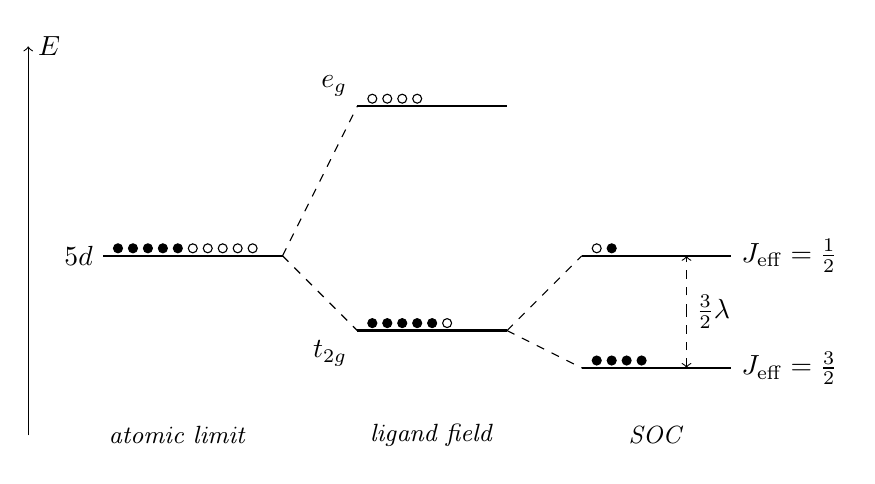
\begin{tikzpicture}[scale=1.9]
 \draw[->] (-0.7,.8) -- (-.7,3.4) node[anchor =  west]{$E$};
 \draw[-,black  ,thick] (-0.2,2)node[anchor=east] {$5d$} -- (1.0,2);
 \foreach \f in {-0.1,0.0,...,0.4} \filldraw (\f,2.05) circle (0.03);
 \foreach \f in {0.4,0.5,...,0.9} \draw (\f,2.05) circle (0.03);
 %
 \draw[-,black,dashed] (1.0,2) -- (1.5,3.0);
 \draw[-,black,dashed] (1.0,2) -- (1.5,1.5);
 %
 \draw[-,black  ,thick] (1.5,3)node[anchor=south east] {$e_g$} -- (2.5,3);
  \foreach \f in {1.6,1.7,...,1.9} \draw (\f,3.05) circle (0.03);
 \draw[-,black  ,thick] (1.5,1.5)node[anchor=north east] {$t_{2g}$} -- (2.5,1.5);
  \foreach \f in {1.6,1.7,...,2.0} \filldraw (\f,1.55) circle (0.03);
  \draw (2.1,1.55) circle (0.03);
 %
 \draw[-,black,dashed] (2.5,1.5) -- (3,2.0);
 \draw[-,black,dashed] (2.5,1.5) -- (3,1.25);
 %
  \draw[-,black  ,thick] (3,2.0) -- (4,2.0) node[anchor= west] {$J_{\mathrm{eff}}=\frac12$} ;
  \draw (3.1,2.05) circle(0.03);
  \filldraw (3.2,2.05) circle(0.03);
 \draw[-,black  ,thick] (3,1.25) -- (4,1.25) node[anchor= west] {$J_{\mathrm{eff}}=\frac32$};
  \foreach \f in {3.1,3.2,...,3.4} \filldraw (\f,1.3) circle (0.03);
  \draw[<-,black, dashed] (3.7,1.25) -- (3.7,1.625) node[anchor = west]{$\frac32\lambda$};
  \draw[->,black, dashed] (3.7,1.625) -- (3.7,2);
  \draw (0.3,0.8) node[]{\small{\emph{atomic limit}}};
  \draw (2.0,0.8) node[]{\small{\emph{ligand field}}};
  \draw (3.5,0.8) node[]{\small{\emph{SOC}}};
 \end{tikzpicture}
\caption{scheme of the split-up of states due to the crystal field and spin orbit coupling. The circles indicate the available spaces and are filled if occupied.}
\end{center}
 \label{split_states}
\end{figure}

%
The two eigenstates are given by a linear combination of the molecular orbits and spin states,
\begin{equation}
 \ket{J_{\mathrm{eff}} =\frac12, M_{J_{\mathrm{eff}}}= \sigma}
 = 
 \frac{1}{\sqrt{3}} \left( \ket{yz,\sigma} -s_{\sigma} \im \ket{zx,\sigma} -s_{\sigma} \ket{xy,-\sigma} \right).
\end{equation}
%\todo{transformation properties of the ground state}
% possible: construct J_eff first (3/2 and 5/2, the second splitting up to 1/2 and 
%%%%%%%%%%%%%%%%%%%%%%%%%%%%%%%%%%%%%%%%%%%%%%%%%%%%%%%%%%%%%%%%%%%%%%%%%%%%%%%%%%%%%%%%%%%%%%%%%%%%%%%%%%%%%%%%%%%%%%%%%%%%%%%%%%%%%%%%%%%%%%%%%%%%%%%%%%%%%%%%%%%%%%%




%\subsubsection{Relative Orientation Of Octahedra}
% rotation by 11° in Sr$_2$IrO$_4$, corner sharing
% edge sharing in other materials, non 2D setup

\newpage
\section{The Hubbard Model}

So far we considered only ions and their immediate vicinity in limit of infinite separation from each other, i.e. without interactions between different sites in the crystal.
In reality the orbitals will overlap and create thereby the possibility of transitions and interactions.
In this chapter we provide an outline on how to construct a set of localized orthonormal states, that allow us to describe our system in second quantization.


\subsection{Tight Binding Model} % in second quantization

Electrons in iridates are localized, i.e. they are well described by wave functions, which are centred around sites in the crystal and vanish fast as one is moving away. 
In this case, atomic orbitals provide a good starting point. 
Since we are interested in dynamics at low temperatures we restrict ourself to the $J=\frac12$ orbital, that is situated at the Fermi level. 
Other orbitals are either completely filled or well above the Fermi level and therefore not important in the dynamics of the system at low temperatures.


We denote the $n$th orbital of the unit cell at site $\vec R_i$ with $\ket{\phi_I} = \phi^n(\vec r - \vec R_i)$.
$I=(n,i)$ is the combined index of orbital number $n$ and site number $i$. $n$ runs over the relevant orbitals of all atoms in the unit cell. 
%
Even though the orbitals are localized, we have a non-zero overlap for different $I=(i,n)$ and $J=(j,m)$, $\braket{\phi_I}{\phi_J} = S_{IJ}\ne \delta_{IJ}$.
This includes overlap in the unit cell and across sites. 
%
The potential in the Hamiltonian is now the sum over atomic potentials at all sites, and the total single-particle Hamiltonian reads
\begin{IEEEeqnarray}{rCl}
 \hat H &=& \frac{1}{2m}\nabla^2 - \sum_I V^n_{\mathrm{atom}}(\vec r - \vec R_i ) \nonumber \\
 &=& H_{\mathrm{atom}}^n(\vec R_i) - \sum_{J\ne I} V^m_{\mathrm{atom}}(\vec r - \vec R_j )
\end{IEEEeqnarray}
In the last line we grouped the terms belonging to the single atom Hamiltonian at space $\vec R_i$, of which $\ket{\phi_I}$ is an eigenfunction with eigenvalue $E^n$.
This allows us to easily identify different contributions the matrix elements of the Hamiltonian.
\begin{equation}
 \bra{ \phi_I} \hat H \ket{\phi_J} = E^{m}S_{IJ}-\beta^{m}\delta_{IJ} - T_{IJ}
\end{equation}
$\beta^m$ corresponds to a shift of energy, due to the integral over the atomic potentials located on all sites apart $I$,
\begin{equation}
 \beta^m = \int \!\!\dint^3 r \:\: \phi^n(\vec r - \vec R_i)^* \sum_{I^{\prime}\ne I} V^{n^{\prime}}_{\mathrm{atom}}(\vec r - \vec R_{i^{\prime}} ) \phi^n(\vec r - \vec R_i)
\end{equation}
This contribution will be small, since the $\ket{\phi_I}(\vec r)$ is small at $\vec r$ where the potential is big. 
The matrix $T_{IJ}$ consists of all non-diagonal integrals of this type, 
\begin{equation}
 T_{IJ} = \int \!\!\dint^3 r\:   \: \phi^{n*}(\vec r - \vec R_I) \sum_{I^{\prime}\ne I} V^{n^{\prime}}_{\mathrm{atom}}(\vec r - \vec R_{i^{\prime}} ) \phi^m(\vec r - \vec R_j)
\end{equation}
if $I \ne J$ and 0 otherwise. 
The biggest contribution in the sum comes from the term with $I^{\prime}=J$, since one wave function has a central overlap with the potential.

We want to transform our basis states such, that they are orthonormal but still located around lattice sites.
Functions of this type are the Wannier functions $\Psi_I$. They are given by the Fourier transformation of Bloch functions.
\begin{equation}
 \Psi_I \left( \vec{r} \right) = \frac1{\sqrt{N}} \sum_{\vec{k}} \euler^{\im \vec{k}\vec{R}_i } \Psi_K(\vec r) 
\end{equation}
We introduced the combined index for $k$-space as well, $K=(n,\vec k)$
Bloch functions are eigenfunctions of the translation operator of the lattice. 
Under a symmetry translation of the lattice, they will only pick up a phase,
\begin{equation}
 \Psi_{K} \left( \vec{r}+\vec{T}\right) = \euler^{\im \vec{k} \vec{T} } u_{K} \left( \vec{r} \right). \label{BlochDef}
\end{equation}
$\vec T$ is a translation vector of the lattice and $u_{K} \left( \vec{r} \right)$ is a function with the same periodicity as the lattice. 
As eigenfunctions of the translational operator the Bloch states are orthogonal, 
which can also be seen by the completeness relation of $\sum_i \euler^{\im ( \vec k - \vec k^{\prime} ) \vec R_i} = N\delta (\vec k - \vec k^{\prime})$
Since the transformation to Wannier states is a unitary transformation, it follows immediately that they are orthogonal as well.

We can now construct Bloch functions from the atomic functions by means of Bloch sums.
\begin{equation}
  \Psi_K(\vec{r}) = N_K \sum_{i} \euler^{\im \vec{k}\vec{R}_i }  \phi^n(\vec{r}-\vec{R}_i). 
\end{equation}
$N_K$ is a $k$- and $n$-dependent normalization factor, which we choose to be real, since we need only it's absolute value.
\begin{equation}
 N_K^{-2}  = \big| \sum_{i,j} \euler^{\im \vec k (\vec R_i-\vec R_j)}  
 \underbrace{\int \!\! \dint^3 r {\phi^n}^*(\vec r - \vec R_i) \phi^n(\vec r- \vec R_j)}_{S_{(n,i),(n,j)}} \big|
\end{equation}
Constructed in this way, the states fulfil the requirement of \ref{BlochDef}, since
\begin{equation}
 \Psi_{K}(\vec{r}+\vec{T}) 
 = N_{K} \euler^{\im \vec{k} \vec{T} } \sum_{i} \euler^{\im \vec{k} (\vec{R}_i-\vec{T})} \phi^n (\vec{r}-\vec{R}_i+\vec{T}) 
 = N_{K} \euler^{\im \vec{k} \vec{T} } \sum_{i} \euler^{\im \vec{k}\vec{R}_i }  \phi^{n}(\vec{r}-\vec{R}_i), 
\end{equation}
where the second step is simply done by a shift in the sum. 
Using the Bloch sums to construct Wannier functions yields the states we are looking for.
These so called Löwdin orbitals are given by
\begin{equation}
 \ket{\varphi_I} = \sum_{j}  \sum_{\vec k} \euler^{\im \vec k ( \vec R_i - \vec R_j ) } N_k \ket{\phi^J}\delta_{mn} = \sum_{J} \mathbf A_{IJ}\ket{\phi_J}\delta_{mn} .
\end{equation}
We introduced the transformation matrix $\mathbf A$, which can be expressed as a product of matrices itself.
Therefore we write the Fourier transformation as 
$\mathbf U_{IK} = \euler^{\im \vec k \vec R_i}\delta_{mn}$, which is unitarian. 
We rewrite the normalization constant as a diagonal matrix, $\mathbf N_{KK^{\prime}}= N_{K} \delta_{KK^{\prime}}$. 
The inverse is again a diagonal matrix with the inverse elements on the diagonal, which gives
$\mathbf N^{-2} = \mathbf U \mathbf S \mathbf U^*$.
The total expression for $\mathbf A$ is therefore
\begin{equation}
 \mathbf A = \mathbf U(\mathbf U^*\mathbf S\mathbf U)^{-\frac12}\mathbf U^* = \mathbf S^{-\frac12}.
\end{equation}
Finally, we can express the Löwdin states in term of atomic orbitals and their overlaps,
\begin{equation}
 \ket{\varphi_I} = \sum_J (\mathbf S^{-\frac12})_{IJ} \ket{\phi_J}\delta_{mn}.
\end{equation}
The matrix $\mathbf S^{-\frac12}$ is defined by a Taylor series of the matrix $\mathbf S$. 
Therefore they commute and hermitian and $\mathbf S^{-\frac12}$ is hermitian.
Since we have only small off-diagonal elements and 1 on the diagonal, we see that the Löwdin states are still
localized around the centres. 
In the limit of large separations, $\mathbf S$ approaches the identity, and we regain the atomic orbitals.
The main difference between the Löwdin states and the atomic ones are imaginary oscillations, that ensure orthogonality.


We can now express the matrix elements of the Hamiltonian in the new basis.
\begin{IEEEeqnarray}{rCl}
 \bra{ \varphi_I} \hat H \ket{\varphi_J} &=& (E^m-\beta^m)\delta_{IJ} - t_{IJ} \\
 t_{IJ} &=& \left\{ 
 \begin{array}{c@{\quad}l}
 -\beta \mathbf S_{IJ} - (\mathbf{S}^{-\frac12}\mathbf T \mathbf S^{-\frac12})_{IJ} & I \ne J \\
 0 & I=J 
 \end{array} \right. \nonumber 
\end{IEEEeqnarray}
%
The calculation of $t_{IJ}$ requires detailed knowledge about the atomic states and the periodic potential.
They are usually calculated through other approximation schemes, for example the local density approximation (LDA).
In calculations we will use values from the literature, that were fitted to LDA + SO calculations.


\subsubsection{Superexchange}
% and how spin exchanges happen 

The direct hopping terms between iridium orbitals are negligible, since the iridium sites are separated by oxygen ions.
Transitions between iridium sites is still possible, but mediated through the $p$-orbitals of oxygen ions. 
These two step hopping processes are called super exchange and give rise to an anti-ferromagnetic coupling.
We will just sketch how to calculate the main contribution to an effective Ir-Ir hopping.

We pick a subsystem of two $J_{\mathrm{eff}}=\frac12$ orbitals of Ir at lattice sites $i$ and $j$ 
and take only hopping between neighbouring orbitals into account.
From the oxygen ion in between we find a double occupied $p$-orbital in between and denote the hopping parameter $t_p$. 
A scheme can be seen in figure \ref{superexchange}.
%
\begin{figure}
\begin{center}
\begin{tikzpicture}
 \draw[-,thick] (0,0) -- (2,0);
 \draw[-,thick] (4,0) node[anchor = north west ]{$p$} -- (6,0) ;
 \draw[-,thick] (8,0) -- (10,0);
 %
 \draw[->,thick] (.8,-.5) -- (.8,.5);
 \draw[->,thick] (1.2,-.5) -- (1.2,.5);
 %
 \draw[->,thick] (4.8,-.5) -- (4.8,.5);
 \draw[<-,thick] (5.2,-.5) -- (5.2,.5);
 %
 \draw[->,thick, gray] (9,-.5) -- (9,.5);
 %
 \draw[->,dashed] (5.2,.6) .. controls (4.2,1.3) and (2.2,1.3) .. node[above]{1.} (1.2,.6) ;
 \draw[->,dashed] (9,.6) .. controls (8.2,1.3) and (6.2,1.3) .. node[above]{2.} (5.2,.6) ;
\end{tikzpicture}
 \caption{scheme of the two processes leading to superexchange, mediated through a $p$-orbital from the ligands}
 \label{superexchange}
 \end{center}
\end{figure}
%
%
The since this involves two hopping processes to and from the $p$-orbital, we get a factor of $t_p$ each time.
We have to divide by the energy of the intermediate step, which is $U+(E_d-E_p)$.
The effective hopping is then $t=\frac{t_p^2}{U+E_d-E_p}$.

%The diagonal term is still given by the eigenvalues of the atomic Hamiltonian with a shift due to the presence of the other potentials. 
%Since this term is proportional to unity, we can remove this factor from the Hamiltonian by shifting the energy scale.

\subsection{Second Quantization}

Having defined our single particle Hamiltonian in terms of orthonormal wave orbitals, 
we can construct the many particle wave function in terms of creation and annihilation operators. 
The operator $c^{\dagger}_{i,\sigma}$ creates a particle with spin $\sigma$ in the orbital $\ket{\varphi_i}$,
while its hermitian conjugate $c_{i,\dagger}$ removes it.
The particles have an effective spin of $\frac12$ and are therefore fermions. 
We introduce the anti-commutation rules for the creation and annihilation operators at equal times.
\begin{IEEEeqnarray}{rClrCl}
 \Big\{c^{\dagger}_{i,\sigma}\:,\: c_{j,\sigma^{\prime}} \Big\} &=& \delta_{ij} \delta_{\sigma, \sigma^{\prime}} 
 &\qquad
 \Big\{c_{i,\sigma}\:,\: c_{j,\sigma^{\prime}} \Big\} &=& 0 \nonumber \\
 \Big\{c_{i,\sigma}^{\dagger}\:,\: c^{\dagger}_{j,\sigma^{\prime}} \Big\} &=& 0 &&& \label{acomm_rules}
\end{IEEEeqnarray}
It follows immediately that  $-c^{\dagger}_{i,\sigma} c^{\dagger}_{j,\sigma} = c^{\dagger}_{j,\sigma} c^{\dagger}_{i,\sigma}$ and $(c^{\dagger}_{i,\sigma})^2 = 0$.
These relations ensure the antisymmetry of the total wave function and thereby the Pauli principle.


% looks like the same thing, but results in oscillations  at the overlapping tails, providing ON.
% Overlap integrals are transformed with that, providing then t_ij
% provides U_ijkl as well?
% see Altmann pp. 177 and 222

%Furthermore they are localized around the positions $\vec{R}_i$.
%Instead of the eigenfunctions of the single particle Hamiltonian, we can use linear combinations of them. 
%This gives us a different set of Wannier functions, that are related to the ones previously defined by another unitary transformation.
%The additional degrees of freedom can be used to optimize the Wannier functions according to certain criteria.
%The most common ones are maximal localization or symmetries of the crystal or the atomic orbitals.
% By taking a relevant subset of atomic states, and defining for each $\vec{k}$
%\begin{equation}
% H_{nm} = \bra{\Psi_{n,\vec{k}}} H \ket{\Psi_{m,\vec{k}}} \text{  and  } S_{nm} = \braket{\Psi_{n,\vec{k}}}{\Psi_{m,\vec{k}}}
%\end{equation}
%we can set up the secular equation
%\begin{equation}
% \det(H_{nm}-E_kS_{nm})=0.
%\end{equation}
%This gives us the band energies. The corresponding eigenstates are called Löwedin functions.
% BAD writing here, tsss. What is the poinit anyway?
% resemble the Löwedin states the crystal symmetry? They should (--> see Slater et al.)



%In this picture we think of electrons as being in a certain state of an atom and hopping to other states rather then being delocalized over the whole crystal.
%In any real system the states will have some overlap, creating the possibility for electrons to hop between different sites.

Creation and annihilation operators can be translated to momentum space as well.
The corresponding operators represent the creation and annihilation operators of the Wannier states. 
\begin{IEEEeqnarray}{rCl}
  c^{\dagger}_{i , \sigma}  =  \frac1{\sqrt N}\sum_{\vec{k}} \euler^{\im \vec{k}\vec{R}_i } c^{\dagger}_{\vec{k} , \sigma}, 
      &\quad&
  c_{i , \sigma}  =  \frac1{\sqrt N} \sum_{\vec{k}} \euler^{-\im \vec{k}\vec{R}_i } c_{\vec{k} , \sigma},  \nonumber\\  
  c^{\dagger}_{\vec{k} , \sigma}  =  \frac1{\sqrt N} \sum_{i} \euler^{-\im \vec{k}\vec{R}_i } c^{\dagger}_{i , \sigma},
    &\quad&
  c_{\vec{k} , \sigma}  =  \frac1{\sqrt N}\sum_{i} \euler^{\im \vec{k}\vec{R}_i } c_{i , \sigma}. \label{FTc}
\end{IEEEeqnarray}
They fulfil the same anti-commutation rules than in the operators in real space.

The single particle Hamiltonian, from now on denoted by $\hat H_0$, reads in second quantization
\begin{IEEEeqnarray}{rCl}
 \hat H_0 
    &=& \sum_{\sigma} \sum_{ij} -t_{ij} \, c^{\dagger}_{i,\sigma} c_{j,\sigma},
\end{IEEEeqnarray}
where $t_{ij}$ are the off-diagonal matrix elements $\bra{\varphi_i} \hat H \ket{\varphi_j}$ defined above.

%
In cases where the tight binding approximation is valid, 
these hopping terms might be very small for large distances between site $i$ and $j$.
As a simplification we restrict the model to close neighbours only, setting all other elements of $\mathbf t$ to zero.
More precisely, we will restrict ourselves to first, second and third nearest neighbours only. 
Due to translational invariance, $t_{ij}$ depends only on the difference $\vec R_i - \vec R_j$.
We further assume isotropy between neighbours in different directions but with the same distance.
Then,  $t_{ij}$ depends only on three parameters,
\begin{equation}
 t_{ij} = \left\{ \begin{array}{l@{\quad}l@{\quad}l}
 t  			& \text{for }\langle i,j\rangle, 					&\text{nearest neighbours} \\ 
 t^{\prime}  		&\text{for } \langle \langle i,j \rangle \rangle, 			&\text{next nearest neighbours} \\
 t^{\prime \prime} 	&\text{for } \langle \langle \langle i , j \rangle \rangle \rangle, 	&\text{ next to next nearest neighbours} 
\end{array} \right.
\end{equation}
and can be expressed as a summation over neighbouring pairs only. 
\begin{IEEEeqnarray}{rCl}
 \hat{H}_0 &=& 
 - t \sum_{\langle i,j \rangle,\sigma} \left( c^{\dagger}_{i,\sigma}c_{j,\sigma} + c^{\dagger}_{j,\sigma}c_{i,\sigma} \right)
 - t^{\prime} \sum_{\langle \langle i,j \rangle \rangle ,\sigma} \left( c^{\dagger}_{i,\sigma}c_{j,\sigma} +c^{\dagger}_{j,\sigma}c_{i,\sigma} \right) \nonumber \\ &&
 - t^{\prime \prime} \sum_{\langle \langle \langle i,j \rangle \rangle \rangle ,\sigma} \left( c^{\dagger}_{i,\sigma}c_{j,\sigma}   + c^{\dagger}_{j,\sigma}c_{i,\sigma} \right)
 -\mu \sum_{i,\sigma} c^{\dagger}_{i,\sigma}c_{i;\sigma}
\end{IEEEeqnarray}
The sums are restricted such, that they count each pair $i,j$ only once. 




\subsection{Band Structure In Momentum Space}




In the simple-most version only nearest neighbour hopping is taken into account, setting $t^{\prime}$ and $t^{\prime \prime}$ to zero.
\begin{equation}
 \hat{H}_0 = - t \sum_{\langle i,j \rangle,\sigma} \left (c^{\dagger}_{i,\sigma}c_{j,\sigma} + c^{\dagger}_{j,\sigma}c_{i,\sigma} \right) 	    -\mu \sum_{i,\sigma} c^{\dagger}_{i,\sigma}c_{i;\sigma}
\end{equation}
In the second term we introduced the chemical potential.
It shows the energetic cost to add a particle to the system.
As an external parameter it can be used to control the particle density $n$, that is the number of particles per site.
$n$ ranges from 0 to 2, since we can occupy each state with at max two particles with opposite spin. 
% \mu = \frac{U}{2} is explained later, when dealing with half filling in greater detail

In order to represent the Hamiltonian in momentum space we insert the relation between the representation of creation and annihilation operators in real space and momentum space,
as stated in equation \ref{FTc}.
%
First, we have a look at the chemical potential term. 
Because of the completeness relation \mbox{$\sum_i \euler^{(\vec{k}-\vec{l})\vec{R}_i } = N\delta_{\vec{k}\vec{l}}$}, it is diagonal in $k$-space as well.
\begin{equation}
 -\mu \sum_{i,\sigma} c^{\dagger}_{i,\sigma}c_{i;\sigma} = 	-\mu \sum_{\vec{k},\sigma} c^{\dagger}_{\vec{k},\sigma}c_{\vec{k}\sigma}
\end{equation}
%
In a similar manner the hopping term turns into	
\begin{IEEEeqnarray}{c}
 -\frac{t}{N} \sum_{\vec k \vec l ,\sigma} \sum_{\langle i,j \rangle } 
	      \left( 
	      \euler^{-\im \left(  \vec{k}\vec{R}_i - \vec{l}\vec{R}_j\right)} c^{\dagger}_{\vec{k},\sigma} c_{\vec l, \sigma}  
	      + \euler^{-\im \left(  \vec{k}\vec{R}_j - \vec{l}\vec{R}_i \right)} c^{\dagger}_{\vec{k},\sigma} c_{\vec l, \sigma} 
	      \right)	      
	      \label{ham_pspace}
\end{IEEEeqnarray}
We can now re-parametrize the sum over nearest neighbours, using the translation vectors $\vec{T}_d$ between nearest neighbours.
$d$ is an index, that runs over all nearest neighbours. 
\begin{equation}
 \sum_{\langle i,j \rangle} = \sum_i \sum_d \quad; \quad \vec{R}_j = \vec{R}_i + \vec{T}_d
\end{equation}

We can therefore write \ref{ham_pspace} as
\begin{IEEEeqnarray}{Cl}
 & -\frac{t}{N} \sum_{\vec{k},\vec{l},\sigma} \sum_{i} \euler^{-\im \left(\vec{k}-\vec{l} \right)\vec{R}_i } 
    \sum_d \left(\euler^{-\im \vec{k}\vec{T}_d} + \euler^{\im  \vec{l} \vec{T}_d} \right) 
    c^{\dagger}_{\vec{k},\sigma}c_{\vec{l},\sigma} \nonumber \\
    =& \sum_{\vec{k},\sigma}  c^{\dagger}_{\vec{k},\sigma}c_{\vec{k},\sigma}  \underbrace{\sum_d -2t \cos( \vec{k} \vec{T}_d ) }_{\varepsilon_{\vec k} }
\end{IEEEeqnarray}
which shows that the single-particle Hamiltonian  is  diagonal in momentum space with the Wannier functions as eigenstates 
and momentum dependent eigenvalues $\varepsilon_{\vec k}$.

In the case of a two dimensional square lattice, the translational vectors of nearest neighbours are given by the lattice constant $a$ times the unit vectors in 
$x$- and $y$-direction, $T_d = a\cdot \vec{e}_d$, $ d \in \{x,y\}$, shown as green arrows in figure \ref{2d_square}.
Using $a$ as the basic length unit, that is $a=1$, 
and normalizing therefore the momentum to the interval $[-\pi,\pi]\times [-\pi,\pi]$ 
we get in this case
\begin{equation}
\varepsilon_{\vec k} = -2t\cos(k_x)-2t\cos(k_y). 
\end{equation}



\begin{figure}
\label{2d_square}
\begin{center}
 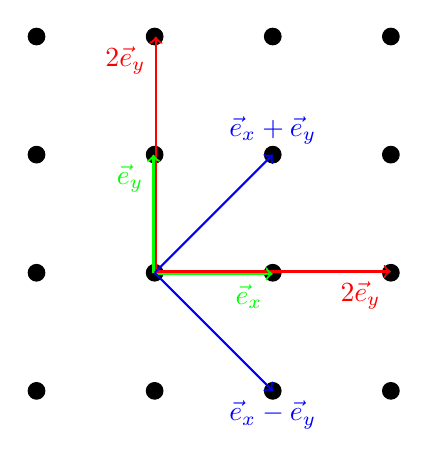
\begin{tikzpicture}[scale=1.5]
 \foreach \x in {1,...,4}
 \foreach \y in {1,...,4}
 \filldraw  (\x,\y) circle (2pt);
 \draw[->,red  ,thick] (2.01,2) -- (2.01,4) node[anchor=north east] {$2\vec e_y$};
 \draw[->,red  ,thick] (2,2.01) -- (4,2.01) node[anchor=north east] {$2\vec e_y$};
 \draw[->,green,thick] (1.99,2) -- (1.99,3) node[anchor=north east] {$\vec e_y$};
 \draw[->,green,thick] (2,1.99) -- (3,1.99) node[anchor=north east] {$\vec e_x$};
 \draw[->,blue ,thick] (2,2) -- (3,3) node[anchor= south] {$\vec e_x+ \vec e_y$};
 \draw[->,blue ,thick] (2,2) -- (3,1) node[anchor=north ] {$\vec e_x- \vec e_y$}; 
 \end{tikzpicture}
\end{center}
\caption{translation vectors $\vec T_d$ in a two dimensional square lattice with first (green), second (blue) and third (red) neighbour interactions}
\end{figure}

The additional term one gets for non-zero second and third neighbour interactions can be treated the same way. 
One has to include the corresponding translational vectors $\vec T_d$ with their respective couplings.
Figure \ref{2d_square} shows the vectors up to third neighbour interactions in the 2D square lattice.
The third neighbours have the same type of translational vectors as the first neighbours, just with twice the length.
The second neighbours are found at $\vec e_x \pm \vec e_y$.
The resulting expression for the energy dispersion in this situation reads
\begin{equation}
 \varepsilon_{\vec k } = -2t \left(\cos k_x + \cos k_y \right) -4t^{\prime} \cos k_x \cos k_y  -2t^{\prime \prime} \left( \cos 2k_x + \cos 2k_y \right)
\end{equation}

We note that the hopping term represents the kinetic energy of particles moving between different sites. 
It is the hopping parameter and the 
geometry of the lattice, that provide the energy dispersion. 
The energy dispersion for Sr$_2$IrO$_4$  with and without next-to-nearest neighbour interactions are shown in figure \ref{fig:energie_dispersion}.



\begin{figure} \centering
\begin{subfigure}{0.49\linewidth} \centering
 \includegraphics[width=\textwidth]{../bandstructure_t.pdf}
 \caption{$ t^{\prime}=t^{\prime \prime} =0$ }
\end{subfigure}
\begin{subfigure}{0.49\linewidth}
  \includegraphics[width=\textwidth]{../bandstructure_ttt.pdf}
  \caption{ $t^{\prime}= 0.2326t$, $t^{\prime \prime} = 0.1163t$}
\end{subfigure}
\caption{single particle energy dispersion in units of t with nesting vector $\vec Q$. }
\label{fig:energie_dispersion}
\end{figure}




\subsection{Hubbard Interaction}

So far we did not take any interactions between particles into account.
The general form of a two particle operator is
\begin{equation}
 H_{\text{int}} = \sum_{\sigma_1 \sigma_2 \sigma_3 \sigma_4} \; \sum_{ijkl} U_{ijkl} \, c^{\dagger}_{i,\sigma_1} c^{\dagger}_{j,\sigma_2} c_{k,\sigma_3} c_{l,\sigma_4}
\end{equation}
%
The matrix elements $U_{ijkl}$ are independent of spin and given by
\begin{equation}
 U_{ijkl} = \int \!  \dint^3 r  \, \dint^3 r^{\prime} \,  \varphi_i^*(\vec{r}) \varphi_j^*(\vec{r}^{\prime}) \frac{e^2}{|\vec{r}-\vec{r}^{\prime} |} \varphi_k(\vec{r}) \varphi_l(\vec{r}) 
\end{equation}
Due to the small overlap of different states $\varphi_i$, only a few matrix elements are of relevant magnitude.
The diagonal matrix elements $U_{iii} = U$ account for the repulsion between electrons on the same site and are certainly the most important contribution.
The fermionic operators ensure the Pauli principle. 
The only non-zero term proportional to $U_{iiii}$ is therefore $c^{\dagger}_{i,\uparrow} c^{\dagger}_{i,\downarrow} c_{i,\uparrow} c_{i,\downarrow}$. 
Using the number operator $n_{i,\sigma} = c^{\dagger}_{i,\sigma} c_{i,\sigma}$, the diagonal interaction term reads
\begin{equation}
 H_{\text{int}} = U \sum_i n_{i,\uparrow} n_{i,\downarrow}.
\end{equation}
Other terms count the interaction of density fluctuations at neighbouring sites through $U_{ijij}$ 
or
the exchange coupling $U_{ijji}$, which yields a Heisenberg like coupling $J_{ij}$.

In the Hubbard model however we take only the diagonal terms $U_{iiii}$ into account.
We choose therefore $U_{ijkl} = \delta_{ijkl} U$. 
Reducing an interaction that is not necessarily local to only on-site interactions is a grave simplification, 
neglecting the vast amount of parameters in the interaction matrix $U_{ijkl}$ and therefore long range repulsion and exchange effects.
As a result, the optimal value for $U$, the only parameter left, does not any longer depend on the integral given above in a simple way.
The interaction seems to be drastically lowered due to screening effects compared to the value one would expect from the correlation integral of the corresponding orbitals
\cite{J.Phys.Cond.Matter.Vol21.34}.
It is not possible to link the parameter $U$ to a physical quantity directly
and the Hubbard model is therefore not a first principle model. 
$U$ has to be seen as an effective parameter.



% Mott Insulator (band split-up using U)
% How U changes the picture


%The Hubbard model is defined by the Hamiltonian
%\begin{equation}
% \hat{H} = \hat{H}_0
%	   + U \sum_i c^{\dagger}_{i,\uparrow}c_{i,\uparrow} c^{\dagger}_{i,\downarrow}c_{i,\downarrow} 
%	    . \label{Hubbard_space}
%\end{equation}
%with a band structure single particle Hamiltonian $\hat{H}_0$.

\subsubsection{Hubbard Term In Momentum Space}

We can express the interaction term through creation and annihilation operators in momentum space as well. 
The summation over all sites in the transformation yields an overall $\delta$-function of momenta,
\begin{IEEEeqnarray}{rl}
 &\frac{U}{N^2} \sum_{\vec{k}\vec{l}\vec{m}\vec{n}} \sum_i \euler^{-\im (\vec{k}-\vec{l}+\vec{m}-\vec{n})\vec{R}_i } 
    c^{\dagger}_{\vec{k},\uparrow}c_{\vec{l},\uparrow} c^{\dagger}_{\vec{m},\downarrow}c_{\vec{n},\downarrow} \nonumber \\
    =& \frac{U}{N} \sum_{\vec{k}\vec{l}\vec{m}\vec{n}} \delta(\vec{k}-\vec{l}+\vec{m}-\vec{n} )
	c^{\dagger}_{\vec{k},\uparrow}c_{\vec{l},\uparrow} c^{\dagger}_{\vec{m},\downarrow}c_{\vec{n},\downarrow} \nonumber \\
    =& \frac{U}{N} \sum_{\vec{k}\vec{k}^{\prime}\vec{q}}
	c^{\dagger}_{\vec{k},\uparrow}c_{\vec{k}-\vec{q},\uparrow} c^{\dagger}_{\vec{k}^{\prime},\downarrow}c_{\vec{k}^{\prime}+\vec{q},\downarrow} \:.
 \end{IEEEeqnarray}
In the last line we choose a convenient parametrization of momenta. 
The interaction is non-diagonal, but it ensures momentum conversation at each vertex.

The total expression for the Hamiltonian in momentum space reads
 \begin{equation}
  \hat{H} = \sum_{\vec{k},\sigma} \left(\varepsilon_{\vec k} - \mu\right) c^{\dagger}_{\vec{k},\sigma}c_{\vec{k}\sigma} + \frac{U}{N} \sum_{\vec{k}\vec{k}^{\prime}\vec{q}}
	c^{\dagger}_{\vec{k},\uparrow}c_{\vec{k}-\vec{q},\uparrow} c^{\dagger}_{\vec{k}^{\prime},\downarrow}c_{\vec{k}^{\prime}+\vec{q},\downarrow}
 \end{equation} 









\section{Mean Field Equations}

\subsubsection{The Mean-Field Hamiltonian}

We treat the Hubbard model in a perturbative approach at the mean-field level.
The Hubbard term  $H_U$ represents the perturbation.
The two-particle operator can be read as a product of two single particle operators.
We can rewrite any product of two operators $\hat{A}$ and $\hat{B}$ as
\begin{IEEEeqnarray}{rCl}
 \hat{A}\cdot\hat{B} 
		    &=&	 \left(\hat A - \langle \hat A \rangle \right) \left( \hat B -\langle \hat B \rangle \right)
			 +\langle \hat A \rangle \hat B
			 +\langle \hat B \rangle \hat A
			 - \langle \hat A \rangle \langle \hat B \rangle
\end{IEEEeqnarray}
In the mean field approach we neglect the first term on the right hand side –the product of fluctuations around their expectation value– leaving us with
\begin{equation}
  \hat{A}\cdot\hat{B} 
		   \approx 
			 \langle \hat A \rangle \hat B
			 +\langle \hat B \rangle \hat A 
			 - \langle \hat A \rangle \langle \hat B \rangle
\end{equation}
% RPA has nothing to do with this I think…
%
We use this relation on the single particle operators 
$c^{\dagger}_{\vec k,\uparrow}c_{\vec k - \vec q,\uparrow}$
and 
$c^{\dagger}_{\vec k,\downarrow}c_{\vec k + \vec q,\downarrow}$
in the Hubbard term of the Hamiltonian. 
Furthermore, we drop the constant term corresponding to $\langle \hat A \rangle \langle \hat B \rangle$, since a constant in the Hamiltonian will not have any
influence on the dynamic of the system. 
The mean-field approximation of the Hubbard term reads
\begin{equation}
 H_U \stackrel{\mathrm{mf}}{\approx}  \frac{U}{N}
 \sum_{\vec{q}} \sum_{\sigma} 
 \left( \sum_{\vec{p}^{\prime}} \langle c^{\dagger}_{\vec{p}^{\prime},-\sigma} c_{\vec{p}^{\prime}+\vec{q},-\sigma} \rangle \right)
	\sum_{\vec p}  c^{\dagger}_{\vec{p},\sigma} c_{\vec{p}-\vec{q},\sigma}. \label{Hubbard_mean_field}
\end{equation}
The expectation value for the one particle operator is different from zero for only two values of $\vec q$.
First, for $\vec q = 0$ the expression yields the spin dependent filling factor, i.e. the number of particles with spin $\sigma$ in relation to the total number of sites $N$.
\begin{equation}
 n_{\sigma} = \frac1N \sum_{\vec k} \langle c^{\dagger}_{\vec k, \sigma} c_{\vec k, \sigma} \rangle.
\end{equation}
A single  site can be empty or occupied by one particle, since we have spin-$\frac12$ particles. The possible values for $n_{\sigma}$ are therefore restricted to the range $[0,1]$.
The total number density is simply the sum of both spin dependent number densities, $n=n_{\uparrow}+n_{\downarrow}$ 
and ranges from the empty case $n=0$ to 2, corresponding to a situation where each sites is occupied by two particles with opposite spin.

%
%
% meaning of mean-field
%
% symmetry bracking, antiferromagnetic ground state
%
%propagators: diagonal, offdiagonal
%
% validity range of the above assumptions: symmetrie, metal insulator transition; limits and corrections
%
%RPA
%
%
The second contribution comes from $\vec q = (\frac12, \frac12)$.
This vector acts as a nesting vector for the Fermi surface of the band structure. 
The dispersion of a square lattice with only nearest-neighbour interactions 
 %can be divided into two sublattices $A$ and $B$, 
 %such that hopping occurs only from one sublattice to the other.
%and as a 
%The partition in sublattices can be understood as an enlargement of the unit cell, resulting in a reduced Brillouin zone of half the size.
%At the same time, we have now to energy disperions, belonging to each sublattice. 
%
depends only on $\cos(k_x) + \cos(k_y)$.
and is therefore perfectly nested.
That means
$\varepsilon_{\vec k} = -\varepsilon_{\vec k + \vec Q}$ with the nesting vector $\vec Q = (\frac12,\frac12)$ in units of $2\pi$.
The Fermi surface at half filling is in this case a perfect square.
Introducing higher order hopping terms deforms the Fermi surface, but nesting with $\vec Q$ holds on a approximate level for small $t^{\prime}$ and $t^{\prime \prime}$.
The Fermi surfaces together with the nesting vector $\vec Q$ are shown for both cases in \ref{fig:energie_dispersion}.
%
%
%
%$\vec Q$ is the basis vector for antiferromagnetic ordering. 
%This is observed in these materials \todo{how general, which ones} and expected % for what reason?


Nesting with $\vec Q = (\frac 12, \frac12)$ leads to a non-zero expectation value for $\langle c^{\dagger}_{\vec k, \sigma} c_{\vec k + \vec Q ,\sigma}$
and therefore to a symmetry broken ground state with an anti-ferromagnetic moment. 
The staggered magnetization is the order parameter of an anti-ferromagnetic state.
In momentum space it reads
\begin{IEEEeqnarray}{lCl}
 m_{s} &=& m_{s, \uparrow} - m_{s, \downarrow}, \\
 m_{s, \sigma} &=& \frac1N  \sum_i (-1)^i \langle c^{\dagger}_{i,\sigma} c_{i,\sigma} \nonumber \\ &&
 \frac1N \sum_{\vec k} \langle c^{\dagger}_{\vec k , \sigma} c_{\vec k + \vec Q, \sigma} \rangle .
\end{IEEEeqnarray}


In terms of the above defined parameters equation \ref{Hubbard_mean_field} simplifies finally to
\begin{equation}
 \hat H = \sum_{\vec k, \sigma} \left( \varepsilon_{\vec k } - \mu + U n_{-\sigma} \right) c^{\dagger}_{\vec k, \sigma} c_{\vec k ,\sigma}
	  + U m_{s,-\sigma} \sum_{\vec k, \sigma} c^{\dagger}_{\vec k + \vec Q, \sigma} c_{\vec k, \sigma}.
\end{equation}
%
%\begin{equation}
% H_U \approx \sum_{\sigma} \left( U n_{-\sigma} \sum_{\vec{p}} c^{\dagger}_{\vec{p}, \sigma} c_{\vec p, \sigma} 
%	      + \frac{ U m_{s,-\sigma}}2
%			      \sum_{\vec p} \left(  c^{\dagger}_{\vec{p}+\vec Q, \sigma} c_{\vec p, \sigma} 
%	                                          + c^{\dagger}_{\vec{p}       , \sigma} c_{\vec p+ \vec Q, \sigma} \right) \right)
%\end{equation}
%
%\begin{IEEEeqnarray}{rCl}
% H_{\mathrm{mf}} &=
%		\sum_{\vec{p},\sigma} &
%				      \left( \varepsilon_{\vec k} - \mu + U n_{-\sigma} \right) 
%					  c^{\dagger}_{\vec{p},\sigma} c_{\vec{p},\sigma}
%				      +\frac{U}2  m_{s,-\sigma}	 
%					  \left( c^{\dagger}_{\vec{p}+\vec{Q},\sigma} c_{\vec{p},\sigma} +\mathrm{h.c.} %c^{\dagger}_{\vec{p},\sigma} c_{\vec{p}+\vec{Q},\sigma} 
%					  \right)					 
%\end{IEEEeqnarray}
%
We are left with a Hamilton operator consisting only of single particle operators. 
That shows the idea of the mean-field approach, describing non-interacting particles that are exposed to an averaged field.
This field is the result off the sum of all particles in the system. It's value will therefore be influenced by the particles itself.
As a result we have to solve the equations for the fields self-consistently, which will be done in the next section. 
The first term in the above mean-field Hamiltonian represents the mean repulsion due to the equal charge of the electrons.
It is proportional to the number density of particles with opposite spin due to the on-site interaction, that is only possible for particles with opposite spin.
The second term corresponds to the coupling to a staggered magnetic field, that is a magnetic field with an alternating orientation on each site. 
The field strength is proportional to the magnetization of the ground state and given by $Um_s$.

\subsubsection{Mean-Field Propagators}

The mean-field Hamiltonian gives rise to two different propagators.
First we get the diagonal contribution, second an off-diagonal one from the staggered component. 
The propagators are defined by
\begin{IEEEeqnarray}{rCl}
 G_{\vec k}(\tau) &=& -\langle \mathcal{T}_{\tau} c_{\vec k         ,\sigma}(\tau)  c^{\dagger}_{\vec k ,\sigma}(0) \rangle \\
 F_{\vec k}(\tau) &=& -\langle \mathcal{T}_{\tau} c_{\vec k +\vec{Q},\sigma}(\tau)  c^{\dagger}_{\vec k ,\sigma}(0) \rangle \\ \label{Def_Propagator}
\end{IEEEeqnarray}
with the imaginary time ordering operator $\mathcal{T}_{\tau}$, acting on a pair of fermion operators according to
\begin{IEEEeqnarray}{rCl}
 \mathcal{T}_{\tau} \hat{A}(\tau_1) \hat{B}(\tau_2) &=&
 -\Theta(\tau_1-\tau_2)\hat{A}(\tau_1) \hat{B}(\tau_2) + \Theta(\tau_2-\tau_1)\hat{B}(\tau_2) \hat{A}(\tau_1) \nonumber \\
 &=& \left\{ \begin{array}{r@{\text{ for }}l} -\hat{A}(\tau_1) \hat{B}(\tau_2) & \tau_1 \ge \tau_2 \\ \hat{B}(\tau_2) \hat{A}(\tau_1) & \tau_1 < \tau_2 \end{array} \right.
\end{IEEEeqnarray}
%
From this definition follows that $n_\sigma$ and $m_{s,\sigma}$ can be expressed in terms of propagators, namely through
\begin{IEEEeqnarray}{lCl}
 n_{\sigma} &=& \frac1N \sum_{\vec k} \left( 1-G_{\vec k, -\sigma}(0) \right) \label{n_DEF}\\
 m_{s,\sigma} &=& -\frac1N \sum_{\vec k} F_{\vec k, -\sigma}(0)		\label{m_DEF}
\end{IEEEeqnarray}


From the definition of the propagators in \ref{Def_Propagator} and the equation of motion for operators, 
$\frac{\dint}{\dint \tau} \hat{A} = [H,\hat{A}] + \frac{\partial}{\partial_{\tau}} \hat{A}$,
we get the differential equation
\begin{IEEEeqnarray}{rCl}
 \partial_{\tau} G_{\vec k ,\sigma}(\tau) 
 &=&
 \delta(\tau) \langle c_{\vec k ,\sigma}(\tau) c^{\dagger}_{\vec k ,\sigma}(0) + c^{\dagger}_{\vec k ,\sigma}(0) c_{\vec k ,\sigma}(\tau) \rangle \nonumber \\&&
 + \Theta(\tau) \langle [\hat H , c_{\vec k ,\sigma}(\tau)] c^{\dagger}_{ \vec k ,\sigma}(0) \rangle		\nonumber \\ &&
 -  \Theta(-\tau) \langle c^{\dagger}_{ \vec k ,\sigma}(0) [\hat H , c_{\vec k ,\sigma}(\tau)]  \rangle \label{EOM_G}
\end{IEEEeqnarray}
Here we used $\partial_{\tau} \Theta(\tau) = \delta(\tau)$.
The commutators can be evaluated using the identity $[AB,C] = A\{B,C\} - \{A,C\}B$ and the anti-commutation rules for the creation and annihilation operators in
equation \ref{acomm_rules}.
%
This leaves us with
\begin{equation}
 [H,c_{\vec k ,\sigma}(\tau)]=-\left(\varepsilon_{\vec k}-\mu + Un_{-\sigma} \right) c_{\vec k ,\sigma}(\tau) - Um_{s,-\sigma} c_{\vec k +\vec{Q},\sigma}(\tau)
\end{equation}
Putting this back in \ref{EOM_G} together with the definitions for $G$ and $F$, we get
\begin{IEEEeqnarray}{rCl}
  \partial_{\tau} G_{\vec k ,\sigma}(\tau) 
&=&
\delta(\tau)\langle \{c_{\vec k ,\sigma}(\tau),c^{\dagger}_{\vec k ,\sigma}(0)\} \rangle
- \left( \varepsilon_{\vec k }-\mu+ Un_{-\sigma} \right) G_{\vec k ,\sigma}(\tau)  \nonumber \\ &&
 -Um_{s,-\sigma} F_{\vec k ,\sigma}(\tau) \label{EOM_G_II}
\end{IEEEeqnarray}
In a next step we take the Fourier transform of this equation. 
The Fourier transformed propagator is related to the propagator in imaginary time through
\begin{IEEEeqnarray}{rCl}
 G_{\vec k ,\sigma}(\tau) &=& \frac{1}{\beta} \sum_n \euler^{-\im \omega_n \tau} G_{\vec k ,\sigma}(\im \omega_n) \\
 G_{\vec k ,\sigma}(\im \omega_n) &=& \int_0^{\beta} \! \!\dint  \tau \: \euler^{\im \omega_n \tau} G_{\vec k ,\sigma}(\tau)
\end{IEEEeqnarray}
The so called Matsubara frequencies $\omega_n$ are given by $\omega_n = \frac{\pi}{\beta}(2n+1), \; n \! \in \! \mathbb{Z}$.
This ensures the anti-periodicity of fermionic Green's functions, $G(\tau+\beta) = -G(\tau)$.
Transforming equation \ref{EOM_G_II} to momentum space we get
\begin{IEEEeqnarray}{rCl}
 \left( \im \omega_n -\varepsilon_{\vec k } +\mu - Un_{-\sigma} \right) G_{\vec k ,\sigma}(\im \omega_n) = 1 +Um_{s,-\sigma} F_{\vec k ,\sigma}(\im \omega_n)
\end{IEEEeqnarray}
In the same way, starting from $\frac{\dint}{\dint \tau} F_{\vec k ,\sigma}(\tau)$ we get for the off-diagonal propagator
\begin{IEEEeqnarray}{rCl}
 \left( \im \omega_n -\varepsilon_{\vec k +\vec{Q}} +\mu - Un_{-\sigma} \right) F_{\vec k ,\sigma}(\im \omega_n) = Um_{s,-\sigma} G_{\vec k ,\sigma}(\im \omega_n)
\end{IEEEeqnarray}
There is no constant term, since the anti-commutator in \ref{EOM_G_II} is zero for off-diagonal momenta. 
Putting the last two equations together we get the expressions for the propagators
\begin{IEEEeqnarray}{rCl}
 G_{\vec k ,\sigma}(\im \omega_n) &=& \frac{ ( \im \omega_n - \varepsilon_{\vec k +\vec{Q}} + \mu -Un_{-\sigma} )}
			      { ( \im \omega_n - \varepsilon_{\vec k +\vec{Q}} + \mu -Un_{-\sigma} )
			        ( \im \omega_n - \varepsilon_{\vec k }         + \mu -Un_{-\sigma} )
			      - U^2m_{s,-\sigma}^2 } \nonumber \\
 F_{\vec k ,\sigma}(\im \omega_n) &=& \frac{ Um_{s,-\sigma}}
			    { ( \im \omega_n - \varepsilon_{\vec k +\vec{Q}} + \mu -Un_{-\sigma} )
			      ( \im \omega_n - \varepsilon_{\vec k }         + \mu -Un_{-\sigma} )
			      - U^2m_{s,-\sigma}^2 }			      
\end{IEEEeqnarray}
We can rewrite this in a more appealing way by factorizing the denominator of both propagators. 
The poles are located at
\begin{equation}
 E_{\vec k ,\sigma}^{\pm}
 =
 \frac{\varepsilon_{\vec k }+\varepsilon_{\vec k +\vec{Q}}}2 -\mu + Un_{-\sigma}  \pm \sqrt{ \left(\frac{\varepsilon_{\vec k }-\varepsilon_{\vec k +\vec{Q}}}2\right)^2 + U^2m_{s,-\sigma}^2 }
\end{equation}
Note that $E_{\vec k ,\sigma}^{\pm}=E_{\vec k +\vec{Q},\sigma}^{\pm}$, since $\varepsilon_{\vec k +2\vec{Q}}=\varepsilon_{\vec k }$.
Using these expressions the propagators can be expressed as
\begin{IEEEeqnarray}{rCl}
 G_{\vec k ,\sigma}(\im \omega_n) &=& \frac{ \im \omega_n - \varepsilon_{\vec k +\vec{Q}} +\mu -Un_{-\sigma} }
					    { (\im \omega_n - E_{\vec k ,\sigma}^+) (\im \omega_n - E_{\vec k ,\sigma}^-) }
\\
 F_{\vec k ,\sigma}(\im \omega_n) &=& \frac{ Um_{s,-\sigma} }
					    { (\im \omega_n - E_{\vec k ,\sigma}^+) (\im \omega_n - E_{\vec k ,\sigma}^-)}
\end{IEEEeqnarray}
We note that $F_{\vec k,\sigma}$ is invariant under a translation $\vec k \rightarrow \vec k +\vec Q$, 
while $G_{\vec k,\sigma}$ changes depending on the dispersion $\varepsilon_{\vec k}$.


%\begin{IEEEeqnarray}{rCl}
%  G_{\vec{p},\sigma}(\im \omega_n) &=& \frac{ u_{\vec{p}        ,\sigma }}{ (\im \omega_n - E_{\vec{p},\sigma}^+) }
%			+ \frac{ u_{\vec{p}+\vec{Q},\sigma }}{ (\im \omega_n - E_{\vec{p},\sigma}^-) } \\
%  F_{\vec{p},\sigma}(\im \omega_n) &=& \frac{ \tilde{u}_{\vec{p},\sigma }}{ (\im \omega_n - E_{\vec{p},\sigma}^+) }
%			- \frac{ \tilde{u}_{\vec{p},\sigma }}{ (\im \omega_n - E_{\vec{p},\sigma}^-) }
%\end{IEEEeqnarray}
%where $u$ and $\tilde{u}$ are given by
% \begin{IEEEeqnarray}{rCl}
% u_{\vec{p},\sigma} &=& \frac{E_{\vec{p},\sigma}^+ - \varepsilon_{\vec{p}+\vec{Q}} +\mu -Un_{-\sigma} }{E_{\vec{p},\sigma}^+ -E_{\vec{p},\sigma}^-} \\
% \tilde{u}_{\vec{p},\sigma} &=& \frac{Um_{s,-\sigma}}{E_{\vec{p},\sigma}^+ -E_{\vec{p},\sigma}^-}.
% \end{IEEEeqnarray}
% \todo{connection to diagrammatic approach, resolve $1-n_{-\sigma} \stackrel{?}{=} n_{-\sigma}$ issue.} 
% \todo{ How to draw nice diagrams in \LaTeX?}

There is an alternative approach from a diagrammatic point of view, that gives the same differential equation for the propagators.
Following the notation of \cite{PhysRevB.65.132404}, 
we denote the bare propagator $G^0_{\vec k,\sigma}$ by a single line, the mean-field propagators by double lines and the interaction by a dashed line.
The off-diagonal propagator $F_{\vec k ,\sigma}$ is marked with an doubled arrow head.
The diagrams for a self-consistent mean-field approximation are shown in figure \ref{Diagr_Props}. 


\begin{fmffile}{prop}

\fmfcmd{%
style_def dbl_plain_dbl_arrow expr p =
draw_double p;
shrink(1.5);
cfill (harrow (p, 0.8));
cfill (harrow (p, 0.7));
endshrink;
enddef;}

\begin{figure}
 \begin{center}
\begin{IEEEeqnarray}{rCl}
 \parbox{20mm}{
	      \begin{fmfgraph}(20mm,30mm)
		\fmfleft{i1}
		\fmfright{o1}
		\fmf{dbl_plain_arrow}{i1,o1}
	      \end{fmfgraph}
	      }
&=& \parbox{15mm}{\begin{fmfgraph}(15mm,30mm) \fmfleft{i} \fmfright{o} \fmf{plain_arrow}{i,o} \end{fmfgraph}} 
   + \parbox{25mm}{\begin{fmfgraph}(25mm,30mm) \fmfleft{i1} \fmfright{o1} \fmf{plain_arrow}{i1,v1} \fmf{dbl_plain_dbl_arrow}{v1,o1}
					   \fmf{dashes,tension=0}{v2,v1} 	 \fmfforce{0.5w,.8h}{v2}     \fmf{dbl_plain_dbl_arrow}{v2,v2}
                \end{fmfgraph} }
	+    \parbox{25mm}{\begin{fmfgraph}(25mm,30mm) \fmfleft{i1} \fmfright{o1} \fmf{plain_arrow}{i1,v1} \fmf{dbl_plain_arrow}{v1,o1}
					   \fmf{dashes,tension=0}{v2,v1} 	 \fmfforce{0.5w,.8h}{v2}     \fmf{dbl_plain_arrow}{v2,v2} \end{fmfgraph} }
\end{IEEEeqnarray}
 \begin{IEEEeqnarray}{rCl}
 \parbox{20mm}{
	      \begin{fmfgraph}(20mm,30mm)
		\fmfleft{i1}
		\fmfright{o1}
		\fmf{dbl_plain_dbl_arrow}{i1,o1}
	      \end{fmfgraph}
	      }
&=& \parbox{25mm}{\begin{fmfgraph}(25mm,30mm) \fmfleft{i1} \fmfright{o1} \fmf{dbl_plain_dbl_arrow}{i1,v1} \fmf{plain_arrow}{v1,o1}
					   \fmf{dashes,tension=0}{v2,v1} 	 \fmfforce{0.5w,.8h}{v2}     \fmf{dbl_plain_arrow}{v2,v2}
                \end{fmfgraph} }
	+    \parbox{25mm}{\begin{fmfgraph}(25mm,30mm) \fmfleft{i1} \fmfright{o1} \fmf{plain_arrow}{i1,v1} \fmf{dbl_plain_arrow}{v1,o1}
					   \fmf{dashes,tension=0}{v2,v1} 	 \fmfforce{0.5w,.8h}{v2}     \fmf{dbl_plain_dbl_arrow}{v2,v2} \end{fmfgraph} }
\end{IEEEeqnarray} 
\end{center}
\caption{Self consistent mean-field equations for $G_{\vec k, \sigma}$ and $F_{\vec k, \sigma}$.}
\label{Diagr_Props}
\end{figure} 
% 
%
By including only single loops we neglect again the possibility of quantum fluctuations, i.e. there are no interactions with virtual states.
Note that the particles on each site of the interaction have different spins and there is no spin transfer. 
All straight arrows have therefore the same spin, while the propagators forming the loops have the opposite spin.
We reflect the sum up to infinite such interactions by using the mean-field propagator after the interaction. 
%
Self-consistency is achieved by using the mean-field propagators in the loops.
This reflects the fact, that $m_{s,\sigma}$ and $n_{\sigma}$ itself depend on the sum over the respective mean-field propagator.
As a result we have to solve the equations for $m_{s,\sigma}$ and $n_{\sigma}$ iteratively. % CHECK IF THIS SENTENCE APPEARS LATER AGAIN.
%
Inserting the bare propagator ${G^0_{\vec k,\sigma}(\im \omega_n)}=(\im \omega_n +\varepsilon_{\vec k} - \mu)^{-1}$ of the non interacting system
as well as equations \ref{n_DEF} and \ref{m_DEF}
reproduces the above expressions for $G_{\vec k, \sigma}$ and $F_{\vec k ,\sigma}$.





\subsubsection{Validity of Mean-Field Description}
% This should maybe be the first point in the mean-field section
%In order to treat the Hubbard model in the mean-field approach we rely on assumptions. that limit this approach to a certain set of parameters.
% Antiferromagnetic groundstate – low T
% low fluctuations
% Mott insulator
% effect of quantum fluctuations





\section{Observables}

In the chapters above we derived an effective Hamiltonian for the iridates.
Furthermore we introduced the Green's functions of the mean-field approach. 
We can use this formalism now, to calculate observable quantities.
They can be compared to experiments to validate the calculations. 
The interaction parameter $U$ has to be fitted to experiments as well.



\subsubsection{X-Ray and Neutron Scattering Experiments}

The main experimental techniques that resolve the magnetic structure of such materials are inelastic neutron and x-ray scattering experiments.
Neutrons are uncharged and do therefore not  interact with the charges of atoms and electrons in the crystal.
This allows them to penetrate thick probes and to interact well below the surface, which makes measurements of the bulk possible. 
They interact solely through their intrinsic spin with the crystal, 
which makes them good candidates for probing the magnetic excitation spectrum.

During the last two decades, resonant inelastic x-ray scattering (RIXS) became an important alternative.
It uses high energetic photons, whose energy is tuned to be resonant to an atomic transition in the system.
The exited electron is lifted in the bands at the Fermi level, where they can interact with particles close to this band.
When the whole created by the incident photon is filled with some electron from that band, a secondary photon is sent out. 
The secondary photon might have a different energy and momentum due to the dynamics of particles in the relevant band,
which is the reason, that this process is inelastic.


In both cases, neutron and photon scattering,  we can measure the momentum transfer and energy transfer to the probe.
The differential cross section $\frac{\dint^2 \sigma}{\dint \Omega \dint \omega}$ is the distribution of secondary particles with a certain momenta. 
The difference to the momenta of the primary photon is passed to the probe as an excitation.
At basic excitations of the system scattering becomes resonant and the differential cross section has a pole.
The position $(\vec q, \omega)$ of these  poles reveal therefore the  dispersion of magnetic excitations in the material.

\subsubsection{Response Functions}

The reaction to an external distortion of the system is expressed through response functions. 
To introduce a distortion to the system, there has to be some generalized external force $F$, for example an electromagnetic field.
This force might be space and time dependent. 
It needs to be coupled to the system through some interaction term in the Hamiltonian, $\hat H_F = \hat X(F)$ for some operator $\hat X$.
In the simplest case, $X$ is linear in $F$, that is $X = X^{\prime} F$.
A linear dependence provides a good description for week perturbations of the system, that is for $F\rightarrow 0$.
$X^{\prime}$ is then just the first term of an expansion of $X$. 
%
The effect on the system will then be measured by the change in some observable $y=\langle Y \rangle$,
which might coincide with the operator $X^{\prime}$.
%
The response of the system is then completely encoded in the linear response function $\chi$, which depends in $Y$ and $X^{\prime}$, 
but is  independent of the external force $F$.


The dynamic magnetic susceptibility is the linear response function to an external space and time dependent magnetic field $\vec B(\vec r,t)$.
It couples to the  magnetic moment $\vec M$ in the system through $  \int \dint^3 r \hat{\vec M}(\vec r) \vec B(\vec r,t)$.
The distortion is quantified through $ \vec M$ as well.
The magnetic susceptibility is therefore proportional to the expectation value of magnetic structure factor. 
\begin{equation}
\chi^{ab}(\vec q,\omega) = \int \dint \tau \euler^{\im \omega \tau} \langle  M^a(q,\tau) M^b(-\vec q, 0) \rangle 
\end{equation}
Measurements are often performed on a poly-crystals or powder. 
This leads to an average over all spatial directions. 
The effective susceptibility is therefore diagonal with the components
\begin{equation}
 \chi^{ab}_{\mathrm{eff}} = \delta^{ab} \mathrm{Tr}(\chi) = \delta^{ab} \langle \vec M(q,\tau) \vec M(-\vec q, 0) \rangle \label{magnSuscI}
\end{equation}



In the simplest case, when the spin axes are parallel to the global axes, the  $\vec M$ is proportional to the spin $\vec J$. 
The spin operator is a one-particle operator with the components $a=x,y,z$, defined as
\begin{equation}
 J^a(R_i)= J^a_i = \frac12\sum_{\sigma,\sigma^{\prime}} c^{\dagger}_{i,\sigma} \left(\sigma^a \right)_{\sigma\sigma^{\prime}} c_{i,\sigma},
\end{equation}
$\sigma^a$ are the Pauli matrices.
%
The momentum space  representation is
\begin{IEEEeqnarray}{rCl}
J^{a}(\vec q) &=& \frac12\sum_{i} \sum_{\sigma,\sigma^{\prime}}  \euler^{\im \vec q \vec R_i} c^{\dagger}_{i ,\sigma} \left(\sigma^a \right)_{\sigma\sigma^{\prime}} c_{i} \nonumber \\
&=& \frac12\sum_{\vec k} \sum_{\sigma,\sigma^{\prime}} c^{\dagger}_{\vec k, \sigma} \left(\sigma^a \right)_{\sigma\sigma^{\prime}} c_{\vec k + \vec q,\sigma^{\prime}}
\end{IEEEeqnarray}
%

In Sr$_2$IrO$_4$ the octahedra are rotated by $\pm \Theta$ in the $x$-$y$-plane in a staggered pattern.
The octahedron is the frame, in which the spin is defined.
The relation between the magnetic moment, expressed in the global axis of the crystal, and the spin $\vec J_i$  at site $i$ is therefore 
related by a coordinate transformation.
The transformation matrix  at site $i$ is
\begin{equation}
 \vec M_i = \left( \begin{array}{ccc} \cos(\Theta) & -(-1)^i \sin(\Theta) & 0 \\ (-1)^i \sin(\Theta) & \cos(\Theta) & 0 \\ 0&0&1 \end{array} \right) \vec J_i
\end{equation}
As with the staggered magnetization the alternating sign can be expressed through $(-1)^i = \euler^{\im \vec Q \vec R_i}$.
In momentum space, the relation between magnetic moment and spin is therefore
\begin{equation}
 \left( \begin{array}{c} M^x_{\vec q} \\ M^y_{\vec q} \\ M^z_{\vec q} \end{array} \right) = 
-2\mu_b \left( \begin{array}{c} \cos(\Theta) J^x_{\vec q} -\sin(\Theta) J^y_{\vec q + \vec Q} \\ \cos(\Theta) J^y_{\vec q} +\sin(\Theta) J^x_{\vec q + \vec Q} \\ J^z_{\vec q} \end{array} \right) 
\end{equation}
We can replace $\vec M$ in equation \ref{magnSuscI} and get
\begin{IEEEeqnarray}{rCl}
 \chi_{\mathrm{eff}}(\omega,\vec q) &=& \cos^2{\Theta} \left( \chi_J^{xx}(\omega,\vec q)+ \chi_J^{yy}(\omega,\vec q) \right) \nonumber \\ &&
 + \sin^2\Theta \left(\chi_J^{xx} (\omega, \vec q + \vec Q) + \chi_J^{yy}(\omega,\vec p + \vec Q)\right)
 + \chi_J^{zz}
\end{IEEEeqnarray}
Where we introduced the spin susceptibility $\chi_J^{ab}(\tau,\vec q = \langle J^a(\tau,\vec q) J^b(0,\vec q) \rangle$. 
Based on the transformation of Pauli matrices $\sigma^{\pm} = \sigma^x \pm \im \sigma^y$ we get the spin components $J^{\pm}$, 
which fulfil the relation $J^{\pm} = (J^{\mp})^{\dagger}$.
Inserting this relation in the definition shows that
\begin{equation}
 \chi_J^{xx} + \chi_J^{yy} = \chi_J^{+-} + \chi_J^{-+} = 2\chi_J^{+-}
\end{equation}
This reduces the expression for the magnetic susceptibility to 
\begin{equation}
 \chi_{\mathrm{eff}}(\omega, \vec q) = 2\cos^2\Theta \chi_J^{+-}(\omega,\vec q)  + 2\sin^2\Theta\chi_J^{+-}(\omega,\vec q+ \vec Q) + \chi_J^{zz}(\omega, \vec q)
\end{equation}



  




 


The magnetic susceptibility contains also the information about scattering effects. 
The differential scattering cross section is given by the imaginary part of the magnetic susceptibility,
\begin{equation}
\frac{\dint^2 \sigma}{\dint \Omega \dint \omega} = -2\Im \left(\chi(\omega,\vec q)\right).
\end{equation}

\todo{derivation from Fermi's Golden Rule in Appendix}









\subsection{Calculating the Dynamic Magnetic Susceptibility}


We can expand the spin susceptibility in terms of Green's functions. 
We will first calculate the transverse susceptibility $\chi_J^{+-}$, by summing up the relevant diagrams.
The longitudinal component $\chi_J^{zz}$ is then calculated in a similar manner.


%The components of the magnetic susceptibility are defined by
%\begin{equation}
% \chi^{ab}(\tau - \tau^{\prime}) = \sum_{\vec{p}} \left( \sum_{\alpha, \beta} c^{\dagger}_{\vec k, \alpha }(\tau) \left(\sigma^{a}\right)_{\alpha \beta} c_{\vec k , \beta}(\tau)  \right)
%			    \cdot \left(  \sum_{\gamma, \delta} c^{\dagger}_{\vec k, \gamma }(\tau^{\prime}) \left(\sigma^{b}\right)_{\gamma \delta} c_{\vec k , \delta}(\tau^{\prime}) \right)  
%\end{equation}


Expressing $\chi_J^{+-}$ and $\chi_J^{-+}$ in creation and destruction operators gives
\begin{IEEEeqnarray}{rCl}
 \chi^{+-}(\vec q,\omega) &=& \int_0^{\beta} \!\!\dint \tau \euler^{\im \omega \tau} \langle \mathcal{T}_{\tau} S^+(\vec q,\tau) S^-(-\vec q,0) \rangle \nonumber \\
			  &=&\int_0^{\beta} \!\!\dint \tau \euler^{\im \omega \tau} 
			  \sum_{\vec k \vec k^{\prime}} \langle c^{\dagger}_{\vec k,\downarrow}(\tau) c_{\vec k+\vec q, \uparrow}(\tau) 
								    c^{\dagger}_{\vec k^{\prime}+\vec q,\downarrow}(0) c_{\vec k^{\prime},\uparrow}(0) \rangle.
\end{IEEEeqnarray}
As a four point correlation function, it describes the propagation of a particle-hole pair with momentum $\vec q$.
The first order bubble diagrams are shown in figure \ref{bubbles}.


\begin{figure}
\begin{tabular}{ccc}
 \begin{fmfgraph*}(120,45)
  \fmfleft{i1} \fmfright{o1} \fmf{dots_arrow,tension=2,label=$\vec q$}{i1,v1} \fmf{dbl_plain_arrow,left=.35}{v1,v2,v4} 
  \fmf{dbl_plain_arrow,left=.35}{v4,v3,v1} \fmf{dots_arrow,tension=2,label=$\vec q$}{v4,o1}
  \fmfforce{.5w,h}{v2} \fmfforce{.5w,0}{v3} \fmf{dashes,tension=0}{v2,v3}
 \end{fmfgraph*}
 &
 \begin{fmfgraph*}(120,45)
  \fmfleft{i1} \fmfright{o1} \fmf{dots_arrow,tension=2,label=$\vec q$}{i1,v1} \fmf{dbl_plain_arrow,left=.35}{v1,v2,v4} 
  \fmf{dbl_plain_arrow,left=.35}{v4,v3,v1} \fmf{dots_arrow,tension=2,label=$\vec q$}{v4,o1}
  \fmfforce{.5w,h}{v2} \fmfforce{.5w,0}{v3} \fmf{dashes,tension=0}{v2,v3}
 \end{fmfgraph*}
 &
 \begin{fmfgraph*}(120,45)
  \fmfleft{i1} \fmfright{o1} \fmf{dots_arrow,tension=2,label=$\vec q$}{i1,v1} \fmf{dbl_plain_arrow,left=.35}{v1,v2,v4} 
  \fmf{dbl_plain_arrow,left=.35}{v4,v3,v1} \fmf{dots_arrow,tension=2,label=$\vec q$}{v4,o1}
  \fmfforce{.5w,h}{v2} \fmfforce{.5w,0}{v3} \fmf{dashes,tension=0}{v2,v3}
 \end{fmfgraph*}
 \\
 \begin{fmfgraph*}(120,45)
  \fmfleft{i1} \fmfright{o1} \fmf{dots_arrow,tension=2,label=$\vec q$}{i1,v1} \fmf{dbl_plain_dbl_arrow,left=.35}{v1,v2,v4} 
  \fmf{dbl_plain_dbl_arrow,left=.35}{v4,v3,v1} \fmf{dots_arrow,tension=2,label=$\vec q$}{v4,o1}
  \fmfforce{.5w,h}{v2} \fmfforce{.5w,0}{v3} \fmf{dashes,tension=0}{v2,v3}
 \end{fmfgraph*}
 &
 \begin{fmfgraph*}(120,45)
  \fmfleft{i1} \fmfright{o1} \fmf{dots_arrow,tension=2,label=$\vec q$}{i1,v1} \fmf{dbl_plain_arrow,left=.35}{v1,v2,v4} 
  \fmf{dbl_plain_arrow,left=.35}{v4,v3,v1} \fmf{dots_arrow,tension=2,label=$\vec q$}{v4,o1}
  \fmfforce{.5w,h}{v2} \fmfforce{.5w,0}{v3} \fmf{dashes,tension=0}{v2,v3}
 \end{fmfgraph*}
 &
 \begin{fmfgraph*}(120,45)
  \fmfleft{i1} \fmfright{o1} \fmf{dots_arrow,tension=2,label=$\vec q$}{i1,v1} \fmf{dbl_plain_arrow,left=.35}{v1,v2} \fmf{dbl_plain_dbl_arrow,left=.35}{v2,v4} 
  \fmf{dbl_plain_arrow,left=.35}{v4,v3} \fmf{dbl_plain_dbl_arrow,left=.35}{v3,v1} \fmf{dots_arrow,tension=2,label=$\vec q$}{v4,o1}
  \fmfforce{.5w,h}{v2} \fmfforce{.5w,0}{v3} \fmf{dashes,tension=0}{v2,v3}
 \end{fmfgraph*}
 \\
 \begin{fmfgraph*}(120,45)
  \fmfleft{i1} \fmfright{o1} \fmf{dots_arrow,tension=2,label=$\vec q$}{i1,v1} \fmf{dbl_plain_arrow,left=.35}{v1,v2,v4} 
  \fmf{dbl_plain_dbl_arrow,left=.35}{v4,v3,v1} \fmf{dots_arrow,tension=2,label=$\vec q$}{v4,o1}
  \fmfforce{.5w,h}{v2} \fmfforce{.5w,0}{v3} \fmf{dashes,tension=0}{v2,v3}
 \end{fmfgraph*}
 &
 \begin{fmfgraph*}(120,45)
  \fmfleft{i1} \fmfright{o1} \fmf{dots_arrow,tension=2,label=$\vec q$}{i1,v1} \fmf{dbl_plain_dbl_arrow,left=.35}{v1,v2,v4} 
  \fmf{dbl_plain_arrow,left=.35}{v4,v3,v1} \fmf{dots_arrow,tension=2,label=$\vec q$}{v4,o1}
  \fmfforce{.5w,h}{v2} \fmfforce{.5w,0}{v3} \fmf{dashes,tension=0}{v2,v3}
 \end{fmfgraph*} &
 \end{tabular}
 \label{bubbles}
 \caption{first order diagrams contributing to $\chi^{+-}(\vec q, \im \omega_n)$.}
\end{figure}


Taking only ladder and bubble diagrams into account is known as the random phase approximation (RPA) which once again neglects quantum fluctuations. 

The contribution from these fluctuations vanish in the large $N$ limit.
This is due to the fact, that each interaction term brings a factor of $\frac{U}{N}$. 
In the limit of large $N$ this means we have only a relevant contribution, when each of those factors is paired with 
a sum over momenta. Crossing interaction lines restrict the momenta involved such, that there is only one free sum, but multiple interaction lines. 
The contribution of those diagrams are therefore small,

Each step in the ladder consists a product of two propagators, which can be the diagonal one $G_{\vec q, \sigma}$
or the off-diagonal propagator $F_{\vec q, \sigma}$, as well as the interaction term $\frac{U}{N}$ times a delta function. 
The building blocks for the ladder diagrams are listed in table \ref{blocks}.


\begin{table}
\centering
\begin{tabular}{|c|V|c|}
\hline
 $\lambda$ &  
 \begin{fmfgraph}(60,35)
  \fmfleft{i1,i2} \fmfright{o1,o2}  \fmf{dashes,tension=0}{i1,i2} \fmf{phantom}{i1,o1} \fmf{phantom}{i2,o2}
 \end{fmfgraph}
 & $\frac UN$  \\[.8cm]
 %
 $\lambda x$ & 
\begin{fmfgraph*}(60,35)
  \fmfleft{i1,i2} \fmfright{o1,o2}  \fmf{dashes,tension=0}{i1,i2} \fmf{dbl_plain_arrow}{o1,i1} \fmf{dbl_plain_arrow}{i2,o2}
  \fmfv{l=$\uparrow$,l.a=25,l.d=1}{o1}
  \fmfv{l=$\downarrow$,l.a=-25,l.d=1}{o2}
 \end{fmfgraph*}
 & $\frac UN\sum_{\vec k,n^{\prime}} G_{\vec k, \downarrow}(\im \omega_{n^{\prime}}) G_{\vec k +\vec q,\uparrow }(\im \omega_{n^{\prime}} + \im \omega_n)$ \\[.8cm]
 %
 $\lambda y$ &
\begin{fmfgraph*}(60,35)
  \fmfleft{i1,i2} \fmfright{o1,o2}  \fmf{dashes,tension=0}{i1,i2} \fmf{dbl_plain_dbl_arrow}{o1,i1} \fmf{dbl_plain_dbl_arrow}{i2,o2}
  \fmfv{l=$\uparrow$,l.a=25,l.d=1}{o1}
  \fmfv{l=$\downarrow$,l.a=-25,l.d=1}{o2}
 \end{fmfgraph*} 
 & $\frac UN\sum_{\vec k,n^{\prime}} F_{\vec k, \downarrow}(\im \omega_{n^{\prime}}) F_{\vec k +\vec q,\uparrow }(\im \omega_{n^{\prime}} + \im \omega_n)$ \\[.8cm]
 %
 $\lambda z_1$ &
 \begin{fmfgraph*}(60,35)
  \fmfleft{i1,i2} \fmfright{o1,o2}  \fmf{dashes,tension=0}{i1,i2} \fmf{dbl_plain_dbl_arrow}{o1,i1} \fmf{dbl_plain_arrow}{i2,o2}
    \fmfv{l=$\uparrow$,l.a=25,l.d=1}{o1}
  \fmfv{l=$\downarrow$,l.a=-25,l.d=1}{o2}
 \end{fmfgraph*}
 &  $\frac UN\sum_{\vec k,n^{\prime}} G_{\vec k, \downarrow}(\im \omega_{n^{\prime}}) F_{\vec k +\vec q,\uparrow }(\im \omega_{n^{\prime}} + \im \omega_n)$ \\[.8cm]
 %
 $\lambda z_2$ &
 \begin{fmfgraph*}(60,35)
  \fmfleft{i1,i2} \fmfright{o1,o2}  \fmf{dashes,tension=0}{i1,i2} \fmf{dbl_plain_arrow}{o1,i1} \fmf{dbl_plain_dbl_arrow}{i2,o2}
   \fmfv{l=$\uparrow$,l.a=25,l.d=1}{o1}
  \fmfv{l=$\downarrow$,l.a=-25,l.d=1}{o2}
 \end{fmfgraph*}
 &  $\frac UN\sum_{\vec k,n^{\prime}} F_{\vec k, \downarrow}(\im \omega_{n^{\prime}}) G_{\vec k +\vec q,\uparrow }(\im \omega_{n^{\prime}} + \im \omega_n)$ \\
 \hline
\end{tabular}
\label{blocks}
\caption{building blocks of ladder diagrams for $\chi^{+-}(\vec q, \im \omega_n)$}
\end{table}

Momentum conversation at each vertex limits the sum over momenta in each block to $\vec k^{\prime} = \vec k + \vec q$ or $\vec k^{\prime} = \vec k + \vec q + \vec Q$
The second possibility is due to the off-diagonal propagator $F_{\vec k,\sigma}$, that adds $\vec Q$ to the momentum. 
Each block consists of a sum over momenta, we can therefore shift the momentum in the product of propagators without changing the value of the sum.
As mentioned above, only $G_{\vec k,\sigma}$ changes under a shift of $\vec Q$, $F_{\vec k,\sigma}$ however is invariant under such a transformation.
Therefore only $x$ will change it's value for $\vec q \rightarrow \vec q + \vec Q$, in all other situations the sum is unchanged, 
as the transformation can be absorbed in $F_{\vec k,\sigma}$,
We will write $\bar x$ to denote the expression for $x$ with $\vec k - \vec k^{\prime} = \vec q + \vec Q$. 

The infinite sum of bubble diagrams represents a geometric series and has an analytical expression.
In order to deal with the right momenta between upper and lower propagator we rewrite it as a $ 2 \times 2$ matrix equation and pick the value that 
corresponds to having $\vec q$ as the external momentum on both sides of the diagram.
The upper component in this matrix equation corresponds to $\vec k - \vec k^{\prime} = \vec q$, 
while the lower one corresponds to $\vec k -\vec k^{\prime} = \vec q + \vec Q$.
The full equation reads then
\begin{equation}
 \chi_{\mathrm{RPA}}^{+-}(\vec q,\im \omega_n) = 
 \left( \begin{array}{cc} x+y & z_1+z_2 \end{array} \right) \cdot \sum_{m=0}^{\infty} (-\lambda M)^m \cdot \left( \begin{array}{c} -1 \\  \: 0 \end{array} \right)
\end{equation}
with the matrix $M$ combining all the possibilities for one new step in the ladder for each order $m$,
\begin{equation}
M =  \left( \begin{array}{cc} x+y & z_1+z_2 \\
			       z_1+ z_2 & \bar x +  y  \end{array} \right)
\end{equation}
At the end of a ladder diagram however we have to fullfill $\vec k - \vec k^{\prime} = \vec q$. 
The last vector ensures the right external momentum at the end and takes care of the minus sign, arising from the loop.
Using the expression for geometric sums we can express the infinte sum through
\begin{IEEEeqnarray}{l}
 \sum_{m=0}^{\infty} (-\lambda M)^m = \left( \mathbf{1} + \lambda M \right)^{-1}  
 %\\ = \left[ \left(1+\lambda(x+y)\right)\left(1+\lambda(\bar x + \bar y)\right) - (z_1 +z_2)(\bar z_1 + \bar z_2) \right]^{-1} \left(\begin{array}{cc} 1+\lambda(\bar x+\bar y) & -(\bar z_1 + \bar z_2) \\ -(z_1 + z_2) & 1+\lambda(x+y) \end{array} \right) \nonumber
\end{IEEEeqnarray}
The whole expression reads then
\begin{equation}
 \chi_{\mathrm{RPA}}^{+-}(\vec q,\im \omega_n) = 
 \frac{ -(x+y)\left(1+\lambda(\bar x+ y) \right) +\lambda(z_1 + z_2)^2}
 {\left(1+\lambda(x+y)\right)\left(1+\lambda(\bar x + y)\right) - \lambda^2(z_1 +z_2)^2} \label{ladder_sum}
\end{equation}
In order to deal with the infinite Matsubara frequency summation we use the procedure from Appendix \ref{MFS},
as we did for finding $m_s$.
The remaining expression depends then only on $\im \omega_n$.
We are interested in the dependence on real frequencies $\omega$. 
Expression \ref{ladder_sum} posesses poles on the real axis, making a simple replacement of $\im \omega_ n$ with $\omega \in \mathbb{R}$ impossible. 
We perform the analytical continuation $\im \omega_n \rightarrow \omega + \im \eta$ with $\omega, \eta \in \mathbb{R}$ and for a small $\eta >0$.
By choosing $\eta$ to be positive we get the retarded response function. \todo{elaborate on that?}
The expression can then be evaluated by carrying out the sum over the momenta using a small numerical value for $\eta$.
This allows us not only to calculate the imaginary part, a finite value of $\eta$ smoothes the resulting response function.
In general, for a function of the type $(\omega+\im \eta - E)^{-1}$, the imaginary part is 
$\frac{- \eta}{\eta^2 + (\omega-E)^2} \stackrel{\eta \rightarrow 0}{\longrightarrow} \pi \delta(\omega -E)$.
In the actual limit of vanishing $\eta$ we expect a delta function, whose poles might not match the discretized momenta of the grid exactly.
Broadening the delta function ensures to not miss momenta due to a finite sized grid and yields a result closer to actual measurements, 
where the response function also shows a finite line width. 

The position of the poles finally yields the spin-wave dispersion $\omega(\vec q)$.
Furthermore, we expect a continuum at higher energies. 


The longitudinal spin susceptibility consists of particle-hole propagators with equal spin.
This doesn't allow for interactions between particle and hole, but for recombination and creation of a new pair. 
The diagrams are therefore bubbles and not a ladder any more.
Two consecutive bubbles have opposite spin. 


% basic expression for \chi^zz
% diagrams, describe alternating spin
% 
% up down symmetry
% x,y,z_i with equal spins
% inverting the matrix. 
% final expression.

% $\chi^{+-},\chi^{zz}$, why is %\chi^{zz} not important?
% Paper that relates longit to transverse susceptibility. 


% expectation from the formula: \omega(0,0) = 0 , \omega(\frac12,\frac12) = 0 etc.
% for perfect nesting it a short calculation that shows why this is the case. (1+\lambda(x+y)) and (z_1 + z_2) will be zero independently.
% without perfect nesting it should hold as well, but is not that easy to see.
% 
% what about the continuum.

%$A=\Im(C^+)$

\end{fmffile}
 
\subsection{Corrections due to Quantum Fluctuations}
  
The simplifications we made in order to treat the Hubbard model in the mean-field approach,  
eliminate any effects that are caused by quantum fluctuations.
These effects may be small and we are able to cover the main features of the system with our simplified description,
but their effect have to be taken into account, especially when comparing calculations to measurements, where they will always be present.
One example is the staggered magnetization, that is overestimated in the mean-field treatment. 
Fluctuations around the antiferromagnetic ground state act as a distortion to the ordering and lower therefore the expectation value of $m_s$.


Calculating the full corrections is beyond the scope of this thesis, but we can account for some major corrections, that have no complicated dependencies.
For the Heisenberg model, the corrections to the spin-wave-velocity, denoted by $\mathcal{Z}_c$, are well known.
They are given by the higher order terms of the $\frac1S$ expansion. 
The main contribution is independent of momentum and frequency. 
Higher order terms are an order of magnitude smaller and their momentum dependence changes the correction factor by $2\%$ at max.
Usually one uses therefore a constant of $\mathcal{Z}_c=1.18$ value to renormalize the whole spin-wave dispersion \cite{PhysRevB.45.10131}.

We will see that our calculation scheme provides the result of the uncorrected linear spin-wave theory in the limit of large U. 
The fact that the Heisenberg model is the large-$U$ limit of the Hubbard model suggests using the same correction factor.
In reference \cite{PhysRevB.43.3617}, Singh calculated corrections in the Hubbard model, 
given by diagrams corresponding to quantum fluctuations,
and found a value consistent with $\mathcal{Z}_c$.

% example of usage of Z_c in Heisenberg \cite{PhysRevB.43.3617}




% explain Z_c
% justify value, if needed from Singh
% staggered magnetization renormalization?

% what did we leave out:
% non-crossing approximation
% things that are not 1P-irreducible.

 
 
\chapter{Results}

\section{Specifications} %of the Calculation}

For all calculations we use dimensionless quantities. 
Firstly, we set the lattice spacing to unity, $a=1$. 
The resulting momenta are therefore given by $(\frac{2\pi n}{N},\frac{2\pi m}{N})$ for $n,m \in [-\frac N2, \frac N2)$.
Furthermore, we express all energy in units of $t$, reducing the number of free parameters in the Hamiltonian therfore by one.
It depends now on only on the parameters $\nicefrac Ut$, $\nicefrac {\mu}t$ and eventually $\nicefrac{t^{\prime}}t$ and $\nicefrac{t^{\prime \prime}}t$.
Temperatures are scaled accordingly with $k_b=1$.
If not otherwise specified, we use only dimensionless units from now on and we will drop $\nicefrac{\cdot7}{t}$ and write just the corresponding symbol, 
assuming it is in units of $t$.


Since the Hubbard model reduces electron-electron interactions in a very crude manner by taking only on-site interactions into account,
its only free parameter $U$ is treated as an adjustable parameter, without an external reference value from other calculations or measurements.	
For this reason the Hubbard model cannot be seen as a first-principle method \cite{J.Phys.Cond.Matter.Vol21.34},
but rather an effective model, that extends a first principle method – the band structure – by introducing one adjustable parameter.
The value of $U$ in materials is not directly observable, but relates to physical quantities as for example the gap in the electrical excitation spectrum.
% check this maybe. Find evtl. values and compare later.
There are other methods using a Hubbard-like interaction, such as LDA+SO+U calculations.
The $U$ we found can then be compared to the one found through this methods. 
Furthermore it allows us to compare the strength of interaction effects in similar materials in relation to each other.

Numerical calculations were performed in two dimensions due to the layered structure of Sr$_2$IrO$_4$, 
using a grid of size $256\times256$.
As a direct result from the discrete Fourier transformation, we get discrete momenta in the Brillouin zone.
The sum over momenta in Greens functions is therefore restricted to $256\times256$ values.
The magnetic susceptibility $\chi(\vec q,\omega)$ was calculated for different values of $\vec q$.
% path
We choose a path along the symmetry lines of the Brillouin zone, that covers the most interesting features of the dispersion.
Due to symmetry in the band structure energies $\varepsilon_{\vec k}$ and therefore in the energies $E^{\pm}_{\vec k}$ as well,
it is sufficient to restrict oneself to just a quarter of the Brillouin zone.
The most basic dependence on $\vec q$ is through a cosine, $\cos (q_i)$ or $\cos(2q_i)$, that is independent of the sign of the components $q_i$.
%
The path chosen for analysis of $\chi$ is a standard way of presenting calculations and measurements and makes it easy to compare our results to related work.
It covers the diagonal $(\frac12t,\frac12t)$, 
the border of the magnetic Brillouin zone perpendicular to the diagonal, $(\frac14(2-t),\frac14t$, 
the x-direction $(\frac12t,0)$ and the y-direction along the border of the Brillouin zone, $(0,\frac12t)$, with $t$ ranging from 0 to 1.
The path is shown in figure \ref{path}.
\begin{figure}
 \label{path}
 \begin{center}
  \includegraphics[width=.9\textwidth]{../path}
  \caption{path through the Brillouin zone (blue), connecting S-X-M-S-$\Gamma$-X. The grey dotted line is the boundary of the magnetic Brillouine zone.}
 \end{center}
\end{figure}
It connects the points $\Gamma=(0,0)$, M=($\frac12,\frac12$), S$=(\frac14,\frac14)$ and X=($\frac12,0$) in the order S-X-M-S-$\Gamma$-X.

The temperature was set to $T=0.0033$, corresponding to 10K at t=0.258eV.
This is a temperature  typically encountered in low-temperature experiments and was used in the measurements that provide our reference data. 
The Néel temperature for Sr$_2$IrO$_4$ is at about 250K$^{\text{\cite{PhysRevB.49.9198}}}$.
Being far below the Néel temperature is necessary for our assumption of an anti-ferromagnetic ground state.
A low temperature is also needed in order to be able to describe the material with an one-band Hubbard model. 
Comparison of calculations over a wide range of temperatures up to 200K showed no significant dependence on the temperature except for the broadness of peaks.


In the calculation of the magnetic susceptibility $\chi$ we need to shift the frequencies infinitesimally above the real axis, 
in order to get a retarded response function. 
This ensures also that we can relate the imaginary part of $\chi$ to the differential cross section. 
In the calculations we used complex frequencies $\omega^+ = \omega + \im \eta$ with a non-zero but small imaginary part $\eta$. 
Choosing a non-infinitesimal value however smears out the delta function, that arises in the imaginary part.
This can be used to compensate for discretisation effects due to the finite sized grid. 
% don't repeat yourself here, see derivation of $\chi$ in chapter before.
%
The value is rather arbitrary and was chosen small, but big enough to ensure a smooth result for the response function with pronounced features.
Choosing this value to big would wash out the response function, making it hard to analyze.
The frequency dependency of propagators and Greens functions is mostly given by $(\omega^+-E^{\pm}_{\vec k})^{-1}$ and combinations thereof.
As a good starting point we can therefore take the maximum difference in the energies $E^{\pm}$ between to nearby points in the finite sized grid of momenta.
For our simplest dispersion, this occurs for example  between the momenta $\vec k_1 = (\pm \frac14,\pm\frac14)$ and $\vec k_2 = \vec k_1 + (\frac1N,0)$.
As an estimation we can take $U=4$ and $m=0.3$ at half filling as a set of typical values, see the discussion below.
We get $|E^{\pm}_{\vec k_1} - E^{\pm}_{\vec k_2}| = 0.001$.
Finally, we found $\eta=0.005$ to be an optimal value.
This value is of order $10^{-3}$ compared to the maximum $\omega(\vec q)$ encountered for typical values of $U$ used in this thesis.



\section{Staggered Magnetization At Half-Filling}
We need to fix the parameters $n_{\sigma}$ and $m_{s,\sigma}$ of the propagators.
They can be expressed through a sum of propagators itself, as shown in equations \ref{n_DEF} and \ref{m_DEF}.
We are left with a system of four non-linear coupled equations.
By using certain symmetries however, they become decoupled and can be solved in a easier way. 

The number density is controlled by the chemical potential, which is another free parameter of the system.
The effective spin-$\frac12$ states are half-filled, that is $n=1$. 
Because of the symmetry between up and down spins we have furthermore $n_{\uparrow}=n_{\downarrow} = \frac12$
This symmetry is not broken but rather assured by the anti-ferromagnetic ground state.

Due to particle-hole symmetry, the Hamiltonian should be invariant under the replacement 
$c_{\vec k,\sigma} \leftrightarrow c_{\vec k,\sigma}^{\dagger}$
% and $\varepsilon_{\vec k} \rightarrow -\varepsilon_{\vec k}$.
In doing this replacement and using the anti-commutation relations for creation and annihilation operators, the Hamilton operator in momentum space reads
\begin{IEEEeqnarray}{rCl}
 \hat H &=& \sum_{\vec k,\sigma} (-\varepsilon_{\vec k} + \mu) c_{\vec k ,\sigma}^{\dagger} c_{\vec k,\sigma} 
 + \frac UN\sum_{\vec k,\vec k^{\prime}, \vec q} c_{\vec k,\uparrow}^{\dagger}c_{\vec k - \vec q,\uparrow}c_{\vec k^{\prime},\downarrow} c_{\vec k^{\prime} + \vec q,\downarrow} 
 \nonumber \\ &&
 -U\sum_{\vec k} \left( c_{\vec k,\uparrow}^{\dagger}c_{\vec k, \uparrow} +c_{\vec k,\downarrow}^{\dagger}c_{\vec k, \downarrow} \right)
  + \sum_{\vec k} (2\varepsilon_{\vec k} + 2\mu + U) 
\end{IEEEeqnarray}
The energy dispersion for holes is given by $\varepsilon_{\vec k}^{\mathrm{holes}} = -\varepsilon_{\vec k}$ 
and by this replacement we get back the original Hamiltonian plus a constant, that does not change our system.
We can collect terms proportional to the total number of holes or particles, 
$nN= \sum_{\vec k,\sigma} c_{\vec k,\sigma}^{\dagger} c_{\vec k,\sigma}$. 
The pre-factor of this terms corresponds to the chemical potential for holes. 
At half-filling it should be the same as for particles, 
we find therefore
\begin{equation}
 \mu = U-\mu \quad \Rightarrow \quad \mu = \frac{U}2.
\end{equation}
This allows us to insert $\mu = \frac U2$ and $n_{\sigma} = \frac12$ immediately in the half filled case.




We furthermore assume that $m_{s,\uparrow}=-m_{s,\downarrow}$. 
The staggered magnetization may thus be expressed by $m_s=2\sigma \cdot m_{s,\sigma}$.
This relation holds in a perfect anti-ferromagnetic state. 
With double occupied states present, there is also a symmetric contribution to $m_{s,\sigma}$ rather than a asymmetric one.
The expression for $m_{s,\sigma}$ adds $(-1)^i$  whenever a particle with spin $\sigma$ is present at site $i$. 
This is not affected by the simultanious presence of a particle with spin $-\sigma$, which will be counted by $m_{s,-\sigma}$ with the same factor of $(-1)^i$.
However, double occupancies can be expected to be distributed evenly throughout the system. 
Due to the alternating sign for the two sublattices we expect this contributions to cancel in the sum over all points in large systems, 
restoring thereby the antisymmetric relation between $m_{s,\uparrow}$ and $m_{s,\downarrow}$. 

In this situation $F_{\vec k,\sigma}$ depends only by an overall sign on $\sigma$, while $G_{\vec k,\sigma}$ becomes spin independent,
\begin{equation}
 G_{\vec k,\uparrow} = G_{\vec k,\downarrow} \qquad F_{\vec k,\uparrow} =-F_{\vec k,\downarrow}.
\end{equation}




In order to calculate $m_ {s,\sigma}$ we solve equation \ref{m_DEF}, where we can replace $m_{s,\uparrow}$ by $-m_{s,\downarrow}$, as stated above.
We furthermore drop the spin labels on $E_{\vec p,\sigma}^{\pm}$, 
since they depend only on the absolute value of $m_{\sigma}$ and $n_{\uparrow} = n_{\downarrow}$ as mentioned above.
This decouples the two equations with respect to the spin label.
By using the definition of the off-diagonal propagator $F_{\sigma,\vec{p}}$ we end up with
\begin{equation}
 m_{s,\sigma} = \frac1N \sum_{\vec{p}} \sum_{n\in \mathbb{Z}} 
							      \frac { Um_{s,\sigma} }
								    { (\im \omega_n - E_{\vec{p}}^+) (\im \omega_n - E_{\vec{p}})}
\end{equation}
The $m_{s,\sigma}$ on the LHS cancels the one in the RHS, but $E^{\pm}$ is still dependent on $|m_{s,\sigma}|$.
To deal with the summation over the Matsubara frequencies $\im \omega_n$, we use Cauchy's integral theorem as described in \ref{MFS}.
The resulting equation
\begin{equation}
 1= \frac{U}{N}\sum_{\vec{p}} \frac{1}{E_{\vec p}^+ - E_{\vec{p}}^-} \left( \frac{1}{1+\euler^{\beta E_{\vec p}^+}} - \frac{1}{1+\euler^{\beta E_{\vec p}^-}} \right)
\end{equation}
is solved using the Newton-Raphson method.
Figure \ref{ms_nn} shows an example of the behaviour of $m_s$ for different values of $U$. The dispersion in this calculation is based 
on nearest neighbour hopping only, that is $t^{\prime} = t^{\prime \prime} = 0$ on a two-dimensional square lattice.
Introducing non-zero $t^{\prime}$ and $t^{\prime \prime}$ showed the same dependence. 
%
%
\begin{figure}
 \label{ms_nn}
 \includegraphics[width=.9\textwidth]{../stagmag_T10.png}
 \caption{staggered magnetization as function of $\frac Ut$}
 
\end{figure}
%
In the limit of infinite $U$ we get $m_s=1$, corresponding to a fully anti-ferromagnetic ground state. 
The strong repulsive interaction prevents double occupancies, because each of them adds $U$ to the energy of the ground state.
We will find therefore one particle at each site.
At the same time provide virtual states a possibility to further lower the ground state energy.
Virtual hopping is only possible for neighbouring sites, that are occupied by particles with opposite spin,
since the Pauli principle prohibits double occupancies of particles with the same spin.
Therefore, an anti-ferromagnetic ground state is energetically preferable to a ferromagnetic one.

Lowering $U$ yields a lower staggered magnetization, since the energy cost for double occupancy gets lower and might be out-weighted by
the reduce in kinetic energy due to hopping.
%
At some point we will encounter a transition to an unordered metallic ground state with $m_s=0$. 
The closing of the Hubbard gap leads to the transition from the insulating state to a conducting one.
The critical value for this transition is sensitive to the parameters for second- and third-neighbour hoppings, 
even though the dependence of $m_s$ on $U$ above the critical value was identical for non-zero and vanishing $t^{\prime}$ and $t^{\prime \prime}$.
The critical value was reported by \citet{PhysRevB.88.035111} to be in the range $U_c \approx 0.7 - 2.2$.
At this point, our assumption of a Hubbard gap and an anti-ferromagnetic ground state is not valid any more. 
The iterative procedure for $m_s$ is not converging in this situation any longer due to the high sensitivity on the band gap through the factor $(E^p_{\vec k} - E^-_{\vec k})^{-1}$.
This term is proportional to $\frac{1}{Um_s}$ for $\vec k$ for points on the Fermi surface with perfect nesting.
Calculations down to $U=0.5$ show that the staggered magnetization falls off very fast for low $U$, this term diverges therefore in this limit.
The limitation for this calculation appears therefore for numerical reasons, that appear roughly at the value, where the transition to the unordered state occurs. 

After finding $m_{s}$, the expression for $n_{\sigma}$ in terms of the propagator $G_{\vec k,\sigma}$ has also been calculated and found to be $n=\frac12$, 
consistent with the above derived condition for the chemical potential $\mu=\frac U2$ at half-filling.



\section{Large U Limit}

A large $U$ creates an antiferromagnet as mentioned above. 
Hopping at half-filling leads to double occupancies, which are supresed due to their high energetic cost. 
Therefore, the system can be described as an Heisenberg antiferromagnet in this limit.
The Heisenberg Hamiltonian with only nearest neighbour couplings is
\begin{equation}
 \hat H = J \sum_{\langle i,j\rangle} \vec{S}_i \cdot \vec{S}_j,
\end{equation}
which will be antiferromagnetic for positive J. 
\todo{derivation of Heisenberg from Hubbard or reference}
Hopping will be treated as a distortion to the system and yields the interaction of neighbouring spins.

%
% http://user.it.uu.se/~ngssc/ngssc_home/S2M2S2/pavarini1.pdf and notes from Morten
% follow explanation, decide in what to include
% include calculation of limit, independent of above considerations
% how does it extend to higher order couplings, that is J^{\prime} and so on as well as t^{\prime}
%

We will expand our result in terms of $\frac{t^2}{U}$ and compare the resulting spin-wave dispersion to the one gained from a Heisenberg model.
Since we are only interested in the position of the poles in $\chi$, it is sufficient to expand the denominator of equation \ref{ladder_sum} and solving for it's roots,
\begin{equation}
 \left(1+\lambda(x+y)\right)\left(1+\lambda(\bar x + y)\right) - \lambda^2(z_1 +z_2)^2 = 0
\end{equation}
We note first that the term $\lambda y$ is dominant in this limit, since $\lambda y \sim 1$, while $\lambda x \sim \frac1{U^2}$ and $\lambda z_i \sim \frac1U$
for infinite $U$.
Expanding this term
up to first order in  $\frac{t^2}U$ we are left with the dispersion
\begin{equation}\label{DispULimit}
 \omega(\vec q) = \frac{4t^2}{Um_s}\sqrt{4-(\cos q_x+\cos q_y)^2}. 
\end{equation}
This is exactly the spin wave dispersion one gets for linear spin waves in a Heisenberg antiferromagnet, 
with the coupling $J=\frac{4t^2}{Um_s}$.
Deriving the Heisenberg model from the Hubbard model yields $J=\frac{4t^2}{U}$, which differs by a factor of $\frac1{m_s}$ from the coupling we get in this expansion.
The dependence of $m_s$ on $U$ shows, that we get a perfect antiferromagnet with $m_s=1$ for large $U$, 
such that the two couplings will be identical in the case, where this approximations are valid. 
%

Linear spin waves are the first term in an $\frac1S$ expansion of the dispersion in a Heisenberg antiferromagnet.
Higher orders renormalize the spin wave dispersion by allowing for quantum fluctuations.
It was claimed by Peres et al. that the staggered magnetization in the expression for $\omega$ in equation \ref{DispULimit} 
plays the role of this renormalization factor \cite{PhysRevB.65.132404}.
Quantum fluctuations do lower the value of $m_s$, but in the mean-field scheme it tends to 1 for large $\frac Ut$ 
and is unable to provide such corrections in the case of large $U$.

The expression for $\omega(\vec q)$ tells us imediatly, that we get a constant dispersion along the 
boundary of the magnetic Brillouin zone, $\omega(\frac12(1-t), \frac12t) =\mathrm{const.}$ for $t \in [0,1]$.
% say sth. why \omega(\vec q = 0) = \omega(\vec q = \vec Q) = 0 is expected. 
% \omega = 0, \vec q = 0: G^2-F^2 = (G-F)^2 - 2GF; (G-F)^2 = 1, GF = z1 = -z2 or similar
% actually is z_1 = z_2 = 0, 1+\lambda(\bar x +y ) = 0 | \vec q =0


By using a large value for $U$ in our calculations, we get results that agree well with the unrenormalized case.
An example for $U=40$ can be seen in figure \ref{largeU}, together with the corresponding dispersion for linear spin waves.
%
\begin{figure}
 \label{largeU}
 \begin{center}
  \includegraphics[width=\textwidth]{../U40}
  \caption{spin wave dispersion for $U=40$ with linear spin-wave theory as comparison}
 \end{center}
\end{figure}
%
% higher order terms: t*(t/U)^n, n>1.
% Heisenberg with J-J'-J''
  

\section{$t$-$U$-Model}



The main feature is the dispersion along the boundary of the reduced Brillouin zone,
that is along $(\frac{\pi}2,\frac{\pi}2) \rightarrow (\pi,0)$ and the under the given symmetries corresponding lines in the other quadrants.
$\omega(\vec q)$ increases along this line, a feature not present in the in the spin wave expansion of the Heisenberg model.
The difference of $\omega(\frac{\pi}2,\frac{\pi}2)$ and $\omega(\pi,0)$ decreases for larger U as one would expect, since we approach the Heisenberg limit.
As we lower the interaction strength, higher order effects become more important.
They correspond to exchanges over multiple sites, being proportional to $t\cdot(\frac tU)^n$ and become non negligible even for higher $n$.


However, a Hubbard model based on nearest neighbour hopping only is not capable of explaining the dispersion observed in experiments.



% t= .258eV, Temperature
%We used the same $t$ as in the previous situation without second- and third neighbour couplings, i.e. $t^{\prime} = t^{\prime \prime} = 0$, 
%when converting values like the temperature.


\section{$t$-$t^{\prime}$-$t^{\prime \prime}$-$U$-Model}


Taken only nearest neighbour interactions into account, the mean-field model is not capable of reproducing all the observed features of this material.
However, including further interactions up to third neighbours improves the system substantially and provides a good description of the dispersion.

The hopping parameters $t,t^{\prime},t^{\prime \prime}$ were treated as fixed parameters, taken from 
\cite{PhysRevLett.106.136402}.
We use $t$ as the energy unit, the new parameters in the calculations are therefore the ratios $\nicefrac{t^{\prime}}{t}$ and $\nicefrac{t^{\prime \prime}}{t}$


Their values are based on fits to  the three orbital tight binding model in the local density approximation, including spin-orbit coupling (LDA+SO). 
The resulting orbital couplings were then projected on the spin-$\frac12$ subspace, 
providing the effective coupling for neighbouring sites of the one-band single particle Hamiltonian build on the effective $spin-\frac12$ states.
The values used in this thesis were 
%
\begin{center}{
\begin{tabular}
%{|r@{=}l|r@{=}l|r@{=}l|}
%\hline
%$t$ & 0.258eV &
%$t^{\prime}$ & 0.06eV &
%$t^{\prime \prime}$ & 0.03eV \\
%\hline
{|c|c|c|}
\hline
$t$ & $t^{\prime}$ & $t^{\prime \prime}$ \\
\hline
0.258eV & 0.06eV & 0.03eV \\
1 & 0.2326 & 0.1163 \\
\hline
\end{tabular}
}\end{center} 
%
The last line shows the dimensionless ratios.


Normalizing reduces not only the number of parameters, the ratio of neighbour interactions can be measured to a higher precision, while 
their absolute value has some uncertainty.\todo{where from?}
\todo{how it is measured, zone boundary dispersion}






The $t-t^{\prime}-t^{\prime \prime}-$Hubbard model, 
i.e. based on a band structure with next, next-to-next and third neighbour hopping terms 
matches the observed shape of the dispersion relation to a high degree for $U=4.2$.
The value was optimized in several runs, where the match was estimated by guidance of the eye.
After renormalizing the frequencies, the dispersion along the boundary is matched the measurements perfectly.
Furthermore our description of the spin-wave velocity is more accurate around $\vec q = 0$ and by symmetry also at $\vec q = (\frac12,\frac12)$ than the one
provided by a fit of the Heisenberg model with up to third-neighbour couplings $J,J^{\prime},J^{\prime \prime}$. 

Our optimal value for $U$ is substantially lower than the one known used for cuprates, which is usually set to around 8$t_{Cu}$ in cuprates. 
\todo{cuprate $U$ and $t$}.
Such a low value for $U$ would result in a conducting state in cuprates, since it is not sufficient to split the $t_{2g}$ bands. 
In iridates with stronger spin-orbit coupling, we get the insulating state, since the degeneracy is lifted.
This provides smaller bands, for which a smaller $U$ is sufficient.
The metal-insulator takes place at $U \approx 2$, depending on the exact couplings of underlying orbits \cite{PhysRevB.88.035111}.
Electron-electron interactions are therefore the reason that Sr$_2$IrO$_4$ is a Mott insulator. 
\begin{figure}
 \begin{center}
  \includegraphics[width=\textwidth]{../compare42.pdf}
 \caption{ spin wave dispersion for $U=4.2$ (blue) compared to measurements (red) and a up to third neighbour Heisenberg model (green). 
 The figure excluding our calculation is taken from \cite{PhysRevLett.108.177003} and recoloured.} 
 \end{center}
\label{tttU42}
\end{figure}


magnetization for $U=4.2$ is $m_s= 2\cdot 0.355$. Together with the above calculations on the rotated staggered spins, we get a net ferromagnetic moment,
if the staggered pattern is made of spins in the $x$-$y$-plane. As shown in the derivation of the magnetic susceptibility and it's connection to the spin susceptibility
we found that $m = \mu_b \sin \Theta m_s= .0135$. This is very close to the observed value of $0.14 \mu_b$.


continuum
show energy dispersion
explain features from that (e.g. form of continuum boundary)
compare to measurements: extract measurement data, choose same path, set atop each other, find perfect U. Interpretation? Continuum?
compare to J-J'-J'' Heisenberg. Can this explain those features? Advantage of this method


\begin{itemize}
\item elaborate on normalization group scheme? Salmhofer et.al.\cite{RevModPhys.84.299}?
\item show diagrams?
\item even do some calculations?
\end{itemize}



\todo{dependence on $\vec q$?}
%---relate to paper: http://www.theophys.kth.se/~wallin/publications/spin_wave_velocity.pdf (Heisenberg, see printout)


\section{Outlook}

% can be improved: 
% more elaborate quantum corrections
% ways to introduce this into calculations
% 
% can be done:
% extend to other materials
% change filling factor
% more detailed analysis of the continuum, broadness of peaks etc.
























\appendix

\chapter{Mathematical techniques}

\section{Matsubara Frequency Summation} \label{MFS}

In the calculations above we encounter functions of the type 
$ \sum_{n \in \mathbb{Z}} f(\im \omega_n)$.
$f$ is usually a propagator or a function of propagators. 
We require $F$ to vanish fast at infinity, that is $|f(z)|< \frac1z\rightarrow 0$ for $|z|\rightarrow \infty$ 
The Matsubara frequencies can be fermionic or bosonic, depending on the type of operator they describe.
For $n \in \mathbb{Z}$ they are given by
\begin{equation}
 \im \omega_n = \left\{ \begin{array}{l @{\quad}c} (2n+1)\im \frac{\pi }{\beta} & \text{(fermionic)} \\ 2n\im\frac{ \pi}{\beta} & \text{(bosonic)} \end{array} \right.
\end{equation}
The Matsubara frequencies are the poles of the function
\begin{equation}
h(z) = \frac{\beta}{\euler^{\beta z} \pm 1} 
\end{equation}
with the positive sign for fermions and the negative one for bosonic frequencies. 
Using Cauchys integral theorem, we can express the sum over the frequencies as an integral. 
We choose a contour $\gamma_1$ that encloses the imaginary axis counterclockwise in a way, that it avoids any other poles not on the axis.
This means running paralell to the axis on a very small distance and closing it at infinity.
% reference to picture. green?
We can now blow up this countour to a circel with inifinite radius which we shall call $\gamma_2$.
Since the function vanishes fast, the integral will be 0, but we have to pick up the Residual of every pole we encounter in deforming the countour. 
The poles will be encircled clockwise, which gives rise to a minus sign.
% reference to the blown up contour. blue?
In doing so, we get the relation
\begin{IEEEeqnarray}{rCl}
 \sum_{n \in \mathbb Z} f(\im \omega_n) &=& \frac1{2\pi\im} \oint_{\gamma_1} \!\!\dint z \: f(z)\cdot h(z) \nonumber \\
 &=&  \frac1{2\pi\im}\underbrace{\oint_{\gamma_2} \!\! \dint z \: f(z)\cdot h(z)}_{=0} -\sum_{i} f(z_i)\cdot h(z_i) 	\\ 
 && \text{for }i \in \{z\in \mathbb{C} | z\text{ pole of} f\} \nonumber
\end{IEEEeqnarray}



The functions used here usually have poles on the real axis. 
With choosing the contour close enough to the imaginary axis we keep those outside of the enclosed area.
For functions falling off faster than $\frac{1}{|z|^{1+\delta}}$ $(\delta>0)$ as $|z|\rightarrow \infty$ we can blow up the contour to a
circle with infinite radius. The integral will vanish, but we pick up residuals for every pole of $f$.
In total we get
\begin{equation}
 \sum_{n\in\mathbb{Z}} f(\im \omega_n) = \frac{1}{2\pi \im} \int_0 \dint z f(z)\frac{\beta}{1+\euler^{\beta z }} 
 = \sum_{\mathrm{Res}_f} \left. \frac{f(z)\beta}{1+\euler^{\beta z }}\right|_{z=z_{\mathrm{Res}_f}}
\end{equation}

\section{Wick Rotation}

\section{Relation between Differential Cross Section and Spectral Density Function}

% follows Altland and Simons p 388-389

Starting from Fermi's Golden Rule, the scattering rate is given by 
\begin{equation} \label{FGR}
 \frac{\dint^2 \sigma}{\dint \Omega \dint \omega}(\vec q, \omega) = 2\pi \sum_{\beta} \left| \bra{\beta} \hat \rho(\vec q) \ket{0}\right|^2 \delta(\omega - E_{\beta}+E_0).
\end{equation}

\bibliographystyle{plainnat}
\bibliography{masterthesis}

\end{document}
